% This file was converted to LaTeX by Writer2LaTeX ver. 1.0.2
% see http://writer2latex.sourceforge.net for more info
\documentclass[letterpaper]{article}
\usepackage[ascii]{inputenc}
\usepackage[T1]{fontenc}
\usepackage[english,english,spanish]{babel}
\usepackage{amsmath}
\usepackage{amssymb,amsfonts,textcomp}
\usepackage{color}
\usepackage{array}
\usepackage{supertabular}
\usepackage{hhline}
\usepackage{hyperref}
\hypersetup{pdftex, colorlinks=true, linkcolor=blue, citecolor=blue, filecolor=blue, urlcolor=blue, pdftitle=, pdfauthor=Reyna , pdfsubject=, pdfkeywords=}
\usepackage[pdftex]{graphicx}
\newcommand\textsubscript[1]{\ensuremath{{}_{\text{#1}}}}
% Text styles
\newcommand\textstylebibuscitbase[1]{#1}
\newcommand\textstyleFootnoteSymbol[1]{\textsuperscript{#1}}
\newcommand\textstylebibusindexbase[1]{#1}
\newcommand\textstylebibusindexbasei[1]{\textit{#1}}
\newcommand\textstylebibusindexbaseb[1]{\textbf{#1}}
% Outline numbering
\setcounter{secnumdepth}{0}
\makeatletter
\newcommand\arraybslash{\let\\\@arraycr}
\makeatother
% List styles
\newcounter{saveenum}
\newcommand\liststyleLi{%
\renewcommand\labelitemi{{\textbullet}}
\renewcommand\labelitemii{${\circ}$}
\renewcommand\labelitemiii{${\blacksquare}$}
\renewcommand\labelitemiv{{\textbullet}}
}
\newcommand\liststyleWWviiiNumv{%
\renewcommand\theenumi{\arabic{enumi}}
\renewcommand\theenumii{\arabic{enumi}.\arabic{enumii}}
\renewcommand\theenumiii{\arabic{enumi}.\arabic{enumii}.\arabic{enumiii}}
\renewcommand\theenumiv{\arabic{enumi}.\arabic{enumii}.\arabic{enumiii}.\arabic{enumiv}}
\renewcommand\labelenumi{ \theenumi }
\renewcommand\labelenumii{ \theenumii }
\renewcommand\labelenumiii{ \theenumiii }
\renewcommand\labelenumiv{ \theenumiv }
}
\newcommand\liststyleLii{%
\renewcommand\theenumi{\arabic{enumi}}
\renewcommand\theenumii{\arabic{enumii}}
\renewcommand\theenumiii{\arabic{enumiii}}
\renewcommand\theenumiv{\arabic{enumiv}}
\renewcommand\labelenumi{\theenumi.}
\renewcommand\labelenumii{\theenumii.}
\renewcommand\labelenumiii{\theenumiii.}
\renewcommand\labelenumiv{\theenumiv.}
}
\newcommand\liststyleLiii{%
\renewcommand\labelitemi{{\textbullet}}
\renewcommand\labelitemii{{\textbullet}}
\renewcommand\labelitemiii{{\textbullet}}
\renewcommand\labelitemiv{{\textbullet}}
}
\newcommand\liststyleLiv{%
\renewcommand\labelitemi{{\textbullet}}
\renewcommand\labelitemii{${\circ}$}
\renewcommand\labelitemiii{${\blacksquare}$}
\renewcommand\labelitemiv{{\textbullet}}
}
\newcommand\liststyleLv{%
\renewcommand\labelitemi{{\textbullet}}
\renewcommand\labelitemii{{\textbullet}}
\renewcommand\labelitemiii{{\textbullet}}
\renewcommand\labelitemiv{{\textbullet}}
}
\newcommand\liststyleWWviiiNumvii{%
\renewcommand\labelitemi{{\textbullet}}
\renewcommand\labelitemii{{\textbullet}}
\renewcommand\labelitemiii{{\textbullet}}
\renewcommand\labelitemiv{{\textbullet}}
}
\newcommand\liststyleWWviiiNumxi{%
\renewcommand\labelitemi{{\textbullet}}
\renewcommand\labelitemii{${\circ}$}
\renewcommand\labelitemiii{${\blacksquare}$}
\renewcommand\labelitemiv{{\textbullet}}
}
\newcommand\liststyleWWviiiNumiv{%
\renewcommand\labelitemi{{\textbullet}}
\renewcommand\labelitemii{${\circ}$}
\renewcommand\labelitemiii{${\blacksquare}$}
\renewcommand\labelitemiv{{\textbullet}}
}
\newcommand\liststyleWWviiiNumiii{%
\renewcommand\theenumi{\arabic{enumi}}
\renewcommand\theenumii{\arabic{enumii}}
\renewcommand\theenumiii{\arabic{enumiii}}
\renewcommand\theenumiv{\arabic{enumiv}}
\renewcommand\labelenumi{(\theenumi)}
\renewcommand\labelenumii{\theenumii.}
\renewcommand\labelenumiii{\theenumiii.}
\renewcommand\labelenumiv{\theenumiv.}
}
\newcommand\liststyleLvi{%
\renewcommand\labelitemi{{\textbullet}}
\renewcommand\labelitemii{${\circ}$}
\renewcommand\labelitemiii{${\blacksquare}$}
\renewcommand\labelitemiv{{\textbullet}}
}
\newcommand\liststyleLvii{%
\renewcommand\labelitemi{{\textbullet}}
\renewcommand\labelitemii{${\circ}$}
\renewcommand\labelitemiii{${\blacksquare}$}
\renewcommand\labelitemiv{{\textbullet}}
}
\newcommand\liststyleLviii{%
\renewcommand\labelitemi{{\textbullet}}
\renewcommand\labelitemii{${\circ}$}
\renewcommand\labelitemiii{${\blacksquare}$}
\renewcommand\labelitemiv{{\textbullet}}
}
\newcommand\liststyleLix{%
\renewcommand\labelitemi{{\textbullet}}
\renewcommand\labelitemii{${\circ}$}
\renewcommand\labelitemiii{${\blacksquare}$}
\renewcommand\labelitemiv{{\textbullet}}
}
\newcommand\liststyleLx{%
\renewcommand\labelitemi{{\textbullet}}
\renewcommand\labelitemii{${\circ}$}
\renewcommand\labelitemiii{${\blacksquare}$}
\renewcommand\labelitemiv{{\textbullet}}
}
\newcommand\liststyleLxi{%
\renewcommand\labelitemi{{\textbullet}}
\renewcommand\labelitemii{${\circ}$}
\renewcommand\labelitemiii{${\blacksquare}$}
\renewcommand\labelitemiv{{\textbullet}}
}
\newcommand\liststyleLxii{%
\renewcommand\theenumi{\arabic{enumi}}
\renewcommand\theenumii{\arabic{enumii}}
\renewcommand\theenumiii{\arabic{enumiii}}
\renewcommand\theenumiv{\arabic{enumiv}}
\renewcommand\labelenumi{\theenumi.}
\renewcommand\labelenumii{\theenumii.}
\renewcommand\labelenumiii{\theenumiii.}
\renewcommand\labelenumiv{\theenumiv.}
}
\newcommand\liststyleLxiii{%
\renewcommand\theenumi{\arabic{enumi}}
\renewcommand\theenumii{\arabic{enumii}}
\renewcommand\theenumiii{\arabic{enumiii}}
\renewcommand\theenumiv{\arabic{enumiv}}
\renewcommand\labelenumi{(\theenumi)}
\renewcommand\labelenumii{\theenumii.}
\renewcommand\labelenumiii{\theenumiii.}
\renewcommand\labelenumiv{\theenumiv.}
}
\newcommand\liststyleWWviiiNumxvi{%
\renewcommand\labelitemi{{\textbullet}}
\renewcommand\labelitemii{${\circ}$}
\renewcommand\labelitemiii{${\blacksquare}$}
\renewcommand\labelitemiv{{\textbullet}}
}
\newcommand\liststyleWWviiiNumxii{%
\renewcommand\labelitemi{{\textbullet}}
\renewcommand\labelitemii{{\textbullet}}
\renewcommand\labelitemiii{{\textbullet}}
\renewcommand\labelitemiv{{\textbullet}}
}
\newcommand\liststyleWWviiiNumvi{%
\renewcommand\theenumi{\arabic{enumi}}
\renewcommand\theenumii{\arabic{enumii}}
\renewcommand\theenumiii{\arabic{enumiii}}
\renewcommand\theenumiv{\arabic{enumiv}}
\renewcommand\labelenumi{\theenumi.}
\renewcommand\labelenumii{\theenumii.}
\renewcommand\labelenumiii{\theenumiii.}
\renewcommand\labelenumiv{\theenumiv.}
}
\newcommand\liststyleLxiv{%
\renewcommand\labelitemi{{\textbullet}}
\renewcommand\labelitemii{${\circ}$}
\renewcommand\labelitemiii{${\blacksquare}$}
\renewcommand\labelitemiv{{\textbullet}}
}
\newcommand\liststyleLxv{%
\renewcommand\theenumi{\arabic{enumi}}
\renewcommand\theenumii{\arabic{enumii}}
\renewcommand\theenumiii{\arabic{enumiii}}
\renewcommand\theenumiv{\arabic{enumiv}}
\renewcommand\labelenumi{\theenumi.}
\renewcommand\labelenumii{\theenumii.}
\renewcommand\labelenumiii{\theenumiii.}
\renewcommand\labelenumiv{\theenumiv.}
}
\newcommand\liststyleLxvi{%
\renewcommand\theenumi{\arabic{enumi}}
\renewcommand\theenumii{\arabic{enumii}}
\renewcommand\theenumiii{\arabic{enumiii}}
\renewcommand\theenumiv{\arabic{enumiv}}
\renewcommand\labelenumi{\theenumi.}
\renewcommand\labelenumii{\theenumii.}
\renewcommand\labelenumiii{\theenumiii.}
\renewcommand\labelenumiv{\theenumiv.}
}
\newcommand\liststyleLxvii{%
\renewcommand\theenumi{\arabic{enumi}}
\renewcommand\theenumii{\arabic{enumii}}
\renewcommand\theenumiii{\arabic{enumiii}}
\renewcommand\theenumiv{\arabic{enumiv}}
\renewcommand\labelenumi{\theenumi.}
\renewcommand\labelenumii{\theenumii.}
\renewcommand\labelenumiii{\theenumiii.}
\renewcommand\labelenumiv{\theenumiv.}
}
\newcommand\liststyleWWviiiNumviii{%
\renewcommand\theenumi{\arabic{enumi}}
\renewcommand\theenumii{\arabic{enumii}}
\renewcommand\theenumiii{\arabic{enumiii}}
\renewcommand\theenumiv{\arabic{enumiv}}
\renewcommand\labelenumi{\theenumi.}
\renewcommand\labelenumii{\theenumii.}
\renewcommand\labelenumiii{\theenumiii.}
\renewcommand\labelenumiv{\theenumiv.}
}
\newcommand\liststyleWWviiiNumxviii{%
\renewcommand\theenumi{\arabic{enumi}}
\renewcommand\theenumii{\arabic{enumii}}
\renewcommand\theenumiii{\arabic{enumiii}}
\renewcommand\theenumiv{\arabic{enumiv}}
\renewcommand\labelenumi{\theenumi.}
\renewcommand\labelenumii{\theenumii.}
\renewcommand\labelenumiii{\theenumiii.}
\renewcommand\labelenumiv{\theenumiv.}
}
\newcommand\liststyleLxviii{%
\renewcommand\labelitemi{{\textbullet}}
\renewcommand\labelitemii{${\circ}$}
\renewcommand\labelitemiii{${\blacksquare}$}
\renewcommand\labelitemiv{{\textbullet}}
}
\newcommand\liststyleLxix{%
\renewcommand\labelitemi{{\textbullet}}
\renewcommand\labelitemii{${\circ}$}
\renewcommand\labelitemiii{${\blacksquare}$}
\renewcommand\labelitemiv{{\textbullet}}
}
\newcommand\liststyleWWviiiNumx{%
\renewcommand\labelitemi{{\textbullet}}
\renewcommand\labelitemii{${\circ}$}
\renewcommand\labelitemiii{${\blacksquare}$}
\renewcommand\labelitemiv{{\textbullet}}
}
\newcommand\liststyleWWviiiNumxvii{%
\renewcommand\labelitemi{{\textbullet}}
\renewcommand\labelitemii{${\circ}$}
\renewcommand\labelitemiii{${\blacksquare}$}
\renewcommand\labelitemiv{{\textbullet}}
}
\newcommand\liststyleWWviiiNumxv{%
\renewcommand\labelitemi{{\textbullet}}
\renewcommand\labelitemii{${\circ}$}
\renewcommand\labelitemiii{${\blacksquare}$}
\renewcommand\labelitemiv{{\textbullet}}
}
\newcommand\liststyleLxx{%
\renewcommand\labelitemi{{\textbullet}}
\renewcommand\labelitemii{${\circ}$}
\renewcommand\labelitemiii{${\blacksquare}$}
\renewcommand\labelitemiv{{\textbullet}}
}
\newcommand\liststyleLxxi{%
\renewcommand\theenumi{\arabic{enumi}}
\renewcommand\theenumii{\arabic{enumii}}
\renewcommand\theenumiii{\arabic{enumiii}}
\renewcommand\theenumiv{\arabic{enumiv}}
\renewcommand\labelenumi{\theenumi.}
\renewcommand\labelenumii{\theenumii.}
\renewcommand\labelenumiii{\theenumiii.}
\renewcommand\labelenumiv{\theenumiv.}
}
% Page layout (geometry)
\setlength\voffset{-1in}
\setlength\hoffset{-1in}
\setlength\topmargin{2.499cm}
\setlength\oddsidemargin{4.001cm}
\setlength\textheight{22.441cm}
\setlength\textwidth{15.09cm}
\setlength\footskip{0.0cm}
\setlength\headheight{0cm}
\setlength\headsep{0cm}
% Footnote rule
\setlength{\skip\footins}{0.119cm}
\renewcommand\footnoterule{\vspace*{-0.018cm}\setlength\leftskip{0pt}\setlength\rightskip{0pt plus 1fil}\noindent\textcolor{black}{\rule{0.25\columnwidth}{0.018cm}}\vspace*{0.101cm}}
% Pages styles
\makeatletter
\newcommand\ps@Standard{
  \renewcommand\@oddhead{}
  \renewcommand\@evenhead{}
  \renewcommand\@oddfoot{}
  \renewcommand\@evenfoot{}
  \renewcommand\thepage{\arabic{page}}
}
\makeatother
\pagestyle{Standard}
\setlength\tabcolsep{1mm}
\renewcommand\arraystretch{1.3}
% footnotes configuration
\makeatletter
\renewcommand\thefootnote{\arabic{footnote}}
\makeatother
% Non-floating captions
\makeatletter
\newcommand\captionof[1]{\def\@captype{#1}\caption}
\makeatother
\newcounter{Figura}
\renewcommand\theFigura{\arabic{Figura}}
\title{}
\author{Reyna }
\date{2013-12-10}
\begin{document}
\clearpage\setcounter{page}{1}\pagestyle{Standard}


\begin{center}

\includegraphics[width=1.88cm,height=1.469cm]{Capitulo2-img1.jpg}
\end{center}
\begin{center}

\includegraphics[width=1.538cm,height=2.205cm]{Capitulo2-img2.png}
\end{center}

\bigskip


\bigskip


\bigskip


\bigskip


\bigskip

{\centering\selectlanguage{spanish}\sffamily
INSTITUTO POLIT\'ECNICO NACIONAL CENTRO DE INVESTIGACI\'ON EN
COMPUTACI\'ON
\par}


\bigskip


\bigskip


\bigskip


\bigskip

{\centering\selectlanguage{spanish}\sffamily
Similitud l\'exico-sem\'antica en un corpus de textos grande coherente
\par}


\bigskip

{\selectlanguage{spanish}\sffamily
TESIS QUE PARA OBTENER EL GRADO DE}

{\selectlanguage{spanish}\sffamily
DOCTOR EN CIENCIAS DE LA COMPUTACI\'ON PRESENTA}


\bigskip


\bigskip

{\centering\selectlanguage{spanish}\sffamily
Reyna Elia Melara Abarca
\par}


\bigskip


\bigskip


\bigskip


\bigskip


\bigskip

{\centering\selectlanguage{spanish}\sffamily
DIRECTORES DE TESIS:
\par}


\bigskip

{\centering\selectlanguage{spanish}\sffamily
DR. ALEXANDER GELBUKH \textbf{\textit{DRA. SOF\'IA N. GALICIA HARO}}
\par}


\bigskip


\bigskip


\bigskip

{\centering\selectlanguage{spanish}\sffamily
M\'EXICO D.F \ \ \ \ \ \ DICIEMBRE DE 2010
\par}


\bigskip


\bigskip


\bigskip

\section{}
\clearpage\section{}
\setcounter{tocdepth}{10}
\renewcommand\contentsname{\'Indice}
\tableofcontents
\section[]{}
\section{}
\section{}
\section{}
\section{}
\section{}
\section{}
\section{}
\section{}
\section{}
\section{}
\section{}
\section{}
\section{}
\section{}
\section{}
\section{}
\section{}
\section{}
\section{}
\section{}
\clearpage\section[Cap\'itulo 2]{Cap\'itulo 2}
\hypertarget{RefHeading4000985831413}{}\subsection[Trabajo
relacionado]{Trabajo relacionado}
\hypertarget{RefHeading4002985831413}{}\subsubsection[2.1
Introducci\'on: La Wikipedia.]{2.1 Introducci\'on: La Wikipedia.}
\hypertarget{RefHeading4004985831413}{}
\bigskip

{\selectlanguage{spanish}\sffamily
Es un proyecto sin fines de lucro de la Fundaci\'on Wikimedia, que
consiste en una enciclopedia en l\'inea, de libre edici\'on y
consulta.}


\bigskip

{\selectlanguage{spanish}\sffamily
Algunas de sus caracter\'isticas que la han convertido en un recurso en
l\'inea relevante son:}


\bigskip

\liststyleLi
\begin{itemize}
\item {\selectlanguage{spanish}\sffamily
\textstylebibuscitbase{\foreignlanguage{spanish}{su gran tama\~no, con
un \'indice de crecimiento constante,}}}
\item {\selectlanguage{spanish}\sffamily
\textstylebibuscitbase{\foreignlanguage{spanish}{su contenido
semi-estructurado, que se reconoce de alta calidad,}}}
\item {\selectlanguage{spanish}\sffamily
\textstylebibuscitbase{\foreignlanguage{spanish}{es independiente del
dominio,}}}
\item {\selectlanguage{spanish}\sffamily
\textstylebibuscitbase{\foreignlanguage{spanish}{est\'a disponible en
varios idiomas (multiling\"ue)}}}
\item {\selectlanguage{spanish}\sffamily
\textstylebibuscitbase{\foreignlanguage{spanish}{es de acceso libre,
disponible para edici\'on y uso incluso fuera de l\'inea.}}}
\end{itemize}

\bigskip

{\selectlanguage{spanish}\sffamily
Su interfaz de usuario es una aplicaci\'on de software basada en Web,
que se ejecuta en el nivel m\'as alto en una arquitectura LAMP. Se
edita en texto plano por un lenguaje de marcas para estructurar
documentos Wiki, que permiten la creaci\'on de manera simple y adhoc de
documentos de contenido colaborativo. Es independiente del dominio, se
actualiza constantemente y es multiling\"ue. Se gestiona a trav\'es del
software libre y de c\'odigo abierto MediaWiki que permite mantener,
crear, configurar y usar los Wiki.}


\bigskip

{\selectlanguage{spanish}\sffamily
El recurso b\'asico de Wikipedia es un \textit{art\'iculo }(o p\'agina),
que define y describe una entidad o evento, y consiste de un documento
de hipertexto con hiperv\'inculos a otras p\'aginas internas o externas
de Wikipedia (Mihalcea, 2007)\textstylebibuscitbase{. Los art\'iculos
se relacionan con otros art\'iculos a trav\'es de hiperv\'inculos que
son palabras o frases dentro del contenido de cada art\'iculo, de modo
que la informaci\'on se complementa formando una red de art\'iculos y
v\'inculos, los cuales no necesariamente son creados por el mismo
autor.}}


\bigskip

{\selectlanguage{spanish}\sffamily
Estos art\'iculos se van agregando bajo el concepto de colaboraci\'on de
los usuarios, quienes pueden estar geogr\'aficamente distribuidos en
diferentes pa\'ises. La mayor\'ia de estos art\'iculos pueden editarse
libremente.}


\bigskip

{\selectlanguage{spanish}\sffamily
Una de las ventajas de Wikipedia es que la {\textquotedblleft}libertad
de contribuci\'on{\textquotedblright} tiene un impacto positivo, tanto
en aspectos cualitativos, como es el aumento en el n\'umero de
art\'iculos y cuantitativos, como la correcci\'on r\'apida de errores,
que se propicia por tener esta caracter\'istica de ambiente
colaborativo \textstylebibuscitbase{(Mihalcea, 2007)}.}


\bigskip

{\selectlanguage{spanish}\sffamily
Sin embargo, tambi\'en tiene desventajas. Esta misma caracter\'istica de
{\textquotedblleft}libertad de contribuci\'on{\textquotedblright}
genera vicios como la saturaci\'on en algunos art\'iculos, art\'iculos
con v\'inculos que no conducen a informaci\'on relevante, v\'inculos
rotos y falta de seriedad en las fuentes de informaci\'on.}


\bigskip

{\selectlanguage{spanish}\sffamily
Cifras publicadas en Wikipedia indican que para enero de 2010, se
hab\'ian registrado alrededor de 68 millones de visitas a las
Wikipedias (que es como se le denomina al conjunto de las Wikipedias de
diferentes lenguaje), y que cerca de 91,000 usuarios participan
activamente, contribuyendo a la edici\'on de aproximadamente 15,000,000
art\'iculos en m\'as de 270 lenguajes. Durante el 2008, las Wikipedias
de los lenguajes ingl\'es, alem\'an, franc\'es, polaco y japones, en
ese orden, fueron las que reflejaron el mayor n\'umero de ediciones de
art\'iculos.}


\bigskip

{\selectlanguage{spanish}\sffamily
En algunos estudios comparativos sobre las Wikipedias, las versiones en
ingl\'es y en alem\'an indican ser las m\'as robustas y mejor
estructuradas, mientras que la Wikipedia en espa\~nol es menos
confiable, ya que incurre en un sin n\'umero de errores y carece de
fuentes fidedignas de informaci\'on, esto debido a que
{\textquotedblleft}cualquiera puede verla o editarla, sin la
intervenci\'on de moderador alguno, ni la sujeci\'on a ning\'un
filtro...{\textquotedblright} (Maldonado, 2010).}


\bigskip

{\selectlanguage{spanish}\sffamily
En el caso de la Wikipedia en ingl\'es\footnote{Statistics,
http://en.wikipedia.org/wiki/Special:Statistics}, algunas cifras
estad\'isticas a septiembre de 2011, indican lo siguiente
(\tablename~\ref{seq:refTable0}):}



\begin{center}
\begin{minipage}{13.878cm}
\captionof{table}[Datos estad\'isticos de la Wikipedia en
Ingl\'es.]{Datos estad\'isticos de la Wikipedia en Ingl\'es.}
\label{seq:refTable0} [Warning: Image ignored]
% Unhandled or unsupported graphics:
%\includegraphics[width=13.878cm,height=5.108cm]{Capitulo2-img3.svm}
\end{minipage}
\end{center}
{\selectlanguage{spanish}\sffamily
El propio fundador de Wikipedia Jimmy Wales se\~nala:
{\textquotedblleft}A una d\'ecada de distancia, cerca de 400 millones
de personas utilizan Wikipedia y sus sitios hermanos cada mes --
alrededor de la tercera parte del mundo conectado por
Internet\footnote{An appeal from Wikipedia founder Jimmy Wales,
http://wikimediafoundation.org/wiki/Special:LandingCheck?landing\_page=WMFJA1\&language=en\&country=MX\&utm\_source=20101124\_JA011A\_EN\&utm\_medium=sitenotice\&utm\_campaign=20101125JA007}{\textquotedblright}.}

{\selectlanguage{spanish}\sffamily
Como puede observarse, Wikipedia tiene caracter\'isticas interesantes,
como lo son su vasto volumen de contenidos, el n\'umero de usuarios que
la editan y la consultan, lo cual deriva en un comportamiento y
crecimiento din\'amico.}


\bigskip

{\selectlanguage{spanish}\sffamily
Wikipedia constituye tambi\'en un recurso que ha sido ampliamente
utilizado para fines acad\'emicos y de
investigaci\'on\footnote{\foreignlanguage{spanish}{\textrm{Wikipedia:Academic
studies of Wikipedia,
}}\url{http://en.wikipedia.org/wiki/Wikipedia:Wikipedia_in_academic_studies}},
tal es el caso del Procesamiento de Lenguaje Natural (PLN), lo cual se
abordar\'a en el resto de este cap\'itulo.}


\bigskip

\subsubsection{2.2 Estructura de Wikipedia}

\bigskip

{\selectlanguage{spanish}\sffamily
Wikipedia est\'a conformada por millones de art\'iculos, organizados en
categor\'ias. Los art\'iculos se relacionan por medio de
hiperv\'inculos. La mayor\'ia de estos art\'iculos pueden ser editados
libremente.}


\bigskip

{\selectlanguage{spanish}\sffamily
Los art\'iculos son p\'aginas Web. Adem\'as de estas p\'aginas existen
otras que no son de contenidos que tengan entradas bibliogr\'aficas,
sino las que se conocen como p\'aginas administrativas.}


\bigskip

{\selectlanguage{spanish}\sffamily
Las p\'aginas, dependiendo del tipo tienen un formato espec\'ifico, de
manera concreta, todo lo que se incorpore a la Wikipedia debe de
realizarse de acuerdo a las plantillas que la plataforma determina y en
base a las pol\'iticas que al respecto tengan se\~naladas.}


\bigskip

{\selectlanguage{spanish}\sffamily
El contenido de la Wikipedia puede ser descargado de los sitios que
oficialmente tiene disponibles, lo cual permite que sea un recurso
\'util para fines acad\'emicos.}


\bigskip

{\selectlanguage{spanish}\sffamily
De manera formal se puede decir que es un recurso semiestructurado,
constituido por un lado, por componentes bien definidos, como son la
estructura de hiperv\'inculos y la jerarqu\'ia de temas o categor\'ias,
y por otro lado, recursos no estructurados como lo son las colecciones
de texto que de ella se generan.}


\bigskip

\paragraph{2.2.1 Recursos estructurados}

\bigskip

{\selectlanguage{spanish}\sffamily
Se puede considerar que su estructura est\'a altamente organizada en
relaci\'on a las siguientes caracter\'isticas:}


\bigskip

\liststyleWWviiiNumv
\begin{enumerate}
\item {\selectlanguage{spanish}\sffamily
\foreignlanguage{spanish}{Cuenta con un sistema de categor\'ias, cuya
finalidad es organizar los art\'iculos, en el que cada art\'iculo debe
de pertenecer al menos a una categor\'ia. Este sistema se} puede pensar
como un grafo o como tesauro\textstylebibuscitbase{.}}
\item {\selectlanguage{spanish}\sffamily
Art\'iculos, que conforman una red con caracter\'isticas de grafo, los
cuales deben cumplir con un formato establecido (MediaWiki), dividido
en secciones, p\'arrafos y las correspondientes relaciones entre
p\'aginas:}

\begin{enumerate}
\item {\selectlanguage{spanish}\sffamily
\textit{p\'aginas de redireccionamiento} (redirect pages), que
establecen relaciones de sin\'onimos,}
\item {\selectlanguage{spanish}\sffamily
\textit{p\'aginas de desambiguaci\'on}, (disambiguation pages), que
establecen relaciones de hom\'onimos,}
\item {\selectlanguage{spanish}\sffamily
Conjunto de hiperv\'inculos o v\'inculos
internos\foreignlanguage{spanish}{ (internal links), que establecen
relaciones de referencias cruzadas y }que tambi\'en se puede considerar
un grafo similar a la red WWW.}
\end{enumerate}
\item {\selectlanguage{spanish}\sffamily
Informaci\'on contenida en estructuras en forma de listas y tablas:}

\begin{enumerate}
\item {\selectlanguage{spanish}\sffamily
contenido de las p\'aginas,}
\item {\selectlanguage{spanish}\sffamily
listas de v\'inculos p\'agina-a-p\'agina (tablas pagelinks,
categorylinks, imagelinks),}
\item {\selectlanguage{spanish}\sffamily
metadatos de im\'agenes (tablas image y oldimage),}
\item {\selectlanguage{spanish}\sffamily
miscel\'aneas (tablas interwiki y site\_stats).}
\end{enumerate}
\end{enumerate}

\bigskip

\paragraph{2.2.2 Recursos no estructurados}

\bigskip

\liststyleLii
\begin{enumerate}
\item {\selectlanguage{spanish}\sffamily
Texto en formato wiki (wikitext) y metadatos embebidos en XML
disponibles para descarga, en forma de respaldos (dump) de la base de
datos de Wikipedia.}
\item {\selectlanguage{spanish}\sffamily
Archivos est\'aticos en hipertexto, Wikipedia Wikis en formato HTML,
disponibles para descarga, en forma de respaldos (dump).}
\end{enumerate}

\bigskip

{\selectlanguage{spanish}\sffamily
Los archivos en texto plano Wikipedia, suelen contener varios gigabytes
de informaci\'on, que requieren de recursos adecuados tanto de
almacenamiento como de procesamiento.}


\bigskip

\paragraph{2.2.3 Art\'iculos}

\bigskip

{\selectlanguage{spanish}\sffamily
Como ya se mencion\'o, la unidad representativa de la Wikipedia es el
\textit{art\'iculo. }Los art\'iculos tienen una forma y un contenido.
La forma la determina el software de MediaWiki y el contenido se
conforma en co-autor\'ia por una comunidad de usuarios\textit{.}}


\bigskip

\paragraph{2.2.3.1 Formato de los art\'iculos: P\'aginas wiki}

\bigskip

{\selectlanguage{spanish}\sffamily
Los art\'iculos se construyen a trav\'es del navegador de MediaWiki
utilizando un patr\'on de dise\~no conocido como \textit{p\'agina}
\textit{wiki}, por medio de un lenguaje propio conocido como
\textit{wikitexto.}}

{\selectlanguage{spanish}\sffamily
Usualmente las p\'aginas wiki tienen tres
representaciones\footnote{Wiki,
\url{http://es.wikipedia.org/wiki/Wiki}}
(\tablename~\ref{seq:refTable1}):}


\bigskip

\begin{center}
\bottomcaption{P\'aginas y edici\'on.}
\label{seq:refTable1}\tablehead{}
\begin{supertabular}{|m{4.2980003cm}|m{9.087cm}|}
\hline
\centering \selectlanguage{spanish}\itshape C\'odigo fuente &
{\selectlanguage{spanish} Que puede editarse por la comunidad de
usuarios. Formato que se almacena localmente en el servidor.}

\selectlanguage{spanish} Texto plano que puede visualizarse unicamente
por medio de la operaci\'on
{\textquotedblleft}Editar{\textquotedblright}.\\\hline
\centering \selectlanguage{spanish}\itshape C\'odigo HTML &
\selectlanguage{spanish} El utilizado por el servidor para mostrar la
informaci\'on a partir del c\'odigo fuente en tiempo real
({\textquotedblleft}al vuelo{\textquotedblright}).\\\hline
\centering \selectlanguage{spanish}\itshape Plantilla o patr\'on de
dise\~no &
\selectlanguage{spanish} Contiene la disposici\'on y elementos comunes a
todas las p\'aginas\\\hline
\end{supertabular}
\end{center}

\bigskip

{\selectlanguage{spanish}\sffamily
Los usuarios a trav\'es de la interfaz de MediaWiki tienen opciones de
creaci\'on y edici\'on de art\'iculos.}


\bigskip

{\selectlanguage{spanish}\sffamily
Wikipedia tiene registro de los datos de creaci\'on y modificaci\'on de
cada art\'iculo.}

\paragraph[]{\selectlanguage{spanish}\sffamily }
\paragraph[2.2.3.2 Contenido de las P\'aginas wiki:
Art\'iculos]{\selectlanguage{spanish}\sffamily 2.2.3.2 Contenido de las
P\'aginas wiki: Art\'iculos}
\paragraph[]{\selectlanguage{spanish}\sffamily }
{\selectlanguage{spanish}\sffamily
Cada art\'iculo tiene una identificador que lo referencia de manera
un\'ivoca, el cual consiste en una o m\'as palabras separadas por
espacios o guiones bajos y ocasionalmente una explicaci\'on entre
par\'entesis (\tablename~\ref{seq:refTable2}).}


\bigskip

\begin{center}
\bottomcaption{Identificador \'unico de un art\'iculo de Wikipedia.}
\label{seq:refTable2}\tablehead{}
\begin{supertabular}{|m{4.668cm}|m{6.388cm}|}
\hline
\centering \selectlanguage{spanish}\bfseries T\'itulo del art\'iculo &
\centering\arraybslash \selectlanguage{spanish}\bfseries Identificador
\'unico del art\'iculo\\\hline
\centering \selectlanguage{spanish} Pentagonal number theorem &
\centering\arraybslash \selectlanguage{spanish}
Pentagonal\_number\_theorem\\\hline
\centering \selectlanguage{spanish} Partition (number theory) &
\centering\arraybslash \selectlanguage{spanish}
Partition\_function\_(number\_theory)\\\hline
\end{supertabular}
\end{center}

\bigskip

{\selectlanguage{spanish}\sffamily
Los art\'iculos utilizan uno de los recursos m\'as importantes de la
World Wide Web, los \textit{hiperv\'inculos. }Los hiperv\'inculos
pueden ser \textit{internos} o \textit{externos}. Los
\textit{hiperv\'inculos internos }o \textit{v\'inculos internos,
}son\textit{ }art\'iculos que hacen alusi\'on a otras
{\textquotedblleft}entradas enciclop\'edicas{\textquotedblright} a las
que se apunta con hiperv\'inculos, lo cual da origen a un modelo
de\textit{ referencias cruzadas }de los art\'iculos de
Wikipedia\textit{.}}


\bigskip

{\selectlanguage{spanish}\sffamily
Los hiperv\'inculos internos se forman con los identificadores de los
art\'iculos y forma externa del hiperv\'inculo o texto anclado (anchor
text). En el lenguaje de marcas de Wikipedia, los hiperv\'inculos se
forman colocando el texto de la forma externa del hiperv\'inculo entre
doble par\'entesis cuadrados. Se utiliza el s\'imbolo {\textbar} (barra
vertical) cuando la forma externa se vincula a un art\'iculo con un
identificador \'unico diferente (\tablename~\ref{seq:refTable3}).}


\bigskip

\begin{center}
\bottomcaption{Formato de los hiperv\'inculos internos.}
\label{seq:refTable3}\tablehead{}
\begin{supertabular}{|m{5.118cm}|m{3.345cm}|m{5.5150003cm}|}
\hline
\centering \selectlanguage{spanish}\bfseries Lenguaje de marcas de
Wikipedia &
\centering \selectlanguage{spanish}\bfseries Anchor text &
\centering\arraybslash \selectlanguage{spanish}\bfseries URL\\\hline
\selectlanguage{spanish} [[Partition function (number
theory){\textbar}unrestricted partition functions]] &
\selectlanguage{spanish}
\href{http://en.wikipedia.org/wiki/Partition_function_(number_theory)}{unrestricted
partition functions} &
\selectlanguage{spanish}
http://en.wikipedia.org/wiki/Partition\_function\_(number\_theory)\\\hline
\selectlanguage{spanish} [[pentagonal numbers]] &
\selectlanguage{spanish}
\href{http://en.wikipedia.org/wiki/Pentagonal_number}{pentagonal
numbers} &
\selectlanguage{spanish}
http://en.wikipedia.org/wiki/Pentagonal\_numbers\\\hline
\end{supertabular}
\end{center}

\bigskip

{\selectlanguage{spanish}\sffamily
Los hiperv\'inculos externos, son v\'inculos a p\'aginas fuera de la
Wikipedia y en su lenguaje de marcas re forman utilizando par\'entesis
cuadrados y un espacio que separa la URL del nombre del v\'inculo
(\tablename~\ref{seq:refTable4}).}


\bigskip

\begin{center}
\bottomcaption{Formato de los hiperv\'inculos externos.}
\label{seq:refTable4}\tablehead{}
\begin{supertabular}{|m{7.235cm}|m{6.9440002cm}|}
\hline
\centering \selectlanguage{spanish}\bfseries Lenguaje de marcas de
Wikipedia &
\centering\arraybslash \selectlanguage{spanish}\bfseries Forma externa
del hiperv\'inculo externo\\\hline
\selectlanguage{spanish}
[http://www.mathpages.com/home/kmath623/kmath623.htm On
Euler{\textquotesingle}s Pentagonal Theorem] at MathPages &
\selectlanguage{spanish}
\href{http://www.mathpages.com/home/kmath623/kmath623.htm}{On
Euler{\textquotesingle}s Pentagonal Theorem} at MathPages\\\hline
\selectlanguage{spanish} [http://front.math.ucdavis.edu/math.HO/0510054
Euler and the pentagonal number theorem] &
\selectlanguage{spanish}
\href{http://front.math.ucdavis.edu/math.HO/0510054}{Euler and the
pentagonal number theorem}\\\hline
\end{supertabular}
\end{center}

\bigskip

\paragraph{2.2.4 P\'aginas de redireccionamiento}

\bigskip

{\selectlanguage{spanish}\sffamily
Como resultado del ambiente colaborativo de Wikipedia, se tienen algunas
implicaciones. Una de estas es la falta de consistencia respecto al uso
del identificador \'unico para una determinada entidad, lo que da como
resultado las \textit{p\'aginas de redireccionamiento
}(\tablename~\ref{seq:refTable5})\textit{, }que no tienen contenido,
pero redirigen al lector a otro art\'iculo, secci\'on de un art\'iculo
u otra p\'agina, usualmente con un t\'itulo
alternativo\footnote{Wikipedia:Redirect,
http://en.wikipedia.org/wiki/Wikipedia:Redirect.}.}


\bigskip

\begin{center}
\bottomcaption{P\'aginas de redireccionamiento.}
\label{seq:refTable5}\tablehead{}
\begin{supertabular}{|m{5.4360003cm}|m{8.478001cm}|}
\hline
\centering \selectlanguage{spanish}\bfseries Tipo de p\'agina &
\centering\arraybslash \selectlanguage{spanish}\bfseries Ejemplo\\\hline
{\selectlanguage{spanish} \textit{P\'agina de redireccionamiento}:}

\selectlanguage{spanish} Se utilizan para ayudar a los usuarios a
encontrar informaci\'on y mantener organizados los wikis, de modo que
m\'ultiples nombres, abreviaciones, errores de ortograf\'ia o temas
relacionados se dirijan hacia la misma p\'agina. &
{\selectlanguage{spanish} Mathematics}

{\selectlanguage{spanish} {\textquotedbl}Maths{\textquotedbl} and
{\textquotedbl}Math{\textquotedbl} redirect here. For other uses of
{\textquotedbl}Mathematics{\textquotedbl} or
{\textquotedbl}Math{\textquotedbl}, see
\href{http://en.wikipedia.org/wiki/Mathematics_(disambiguation)}{Mathematics
(disambiguation)} and
\href{http://en.wikipedia.org/wiki/Math_(disambiguation)}{Math
(disambiguation)}.}

~

{\selectlanguage{spanish}
\href{http://en.wikipedia.org/wiki/Mathematics}{Mathematics} is the
body of knowledge justified by deductive reasoning about abstract
structures, starting from axioms and definitions.}

{\selectlanguage{spanish} \textbf{Mathematics} may also refer to}

\liststyleLiii
\begin{itemize}
\item \selectlanguage{spanish}
\href{http://en.wikipedia.org/wiki/Mathematics_(producer)}{\textit{Mathematics}}\href{http://en.wikipedia.org/wiki/Mathematics_(producer)}{
(producer)}, a hip-hop producer\item \selectlanguage{spanish}
\href{http://en.wikipedia.org/wiki/Mathematics_(album)}{\textit{Mathematics}}\href{http://en.wikipedia.org/wiki/Mathematics_(album)}{
(album)}, an album by the band The Servant\item
\selectlanguage{spanish}
\href{http://en.wikipedia.org/wiki/Mathematics_(song)}{{\textquotedbl}}\href{http://en.wikipedia.org/wiki/Mathematics_(song)}{\textit{Mathematics}}\href{http://en.wikipedia.org/wiki/Mathematics_(song)}{{\textquotedbl}
(song)}, a song by Mos Def\item \selectlanguage{spanish}
\href{http://en.wikipedia.org/w/index.php?title=Mathematics_(Little_Boots_song)&action=edit&redlink=1}{{\textquotedbl}}\href{http://en.wikipedia.org/w/index.php?title=Mathematics_(Little_Boots_song)&action=edit&redlink=1}{\textit{Mathematics}}\href{http://en.wikipedia.org/w/index.php?title=Mathematics_(Little_Boots_song)&action=edit&redlink=1}{{\textquotedbl}
(Little Boots song)}, a song by
\href{http://en.wikipedia.org/wiki/Little_Boots}{Little Boots}\item
\selectlanguage{spanish}
\href{http://en.wikipedia.org/wiki/Mathematics_Magazine}{\textit{Mathematics
Magazine}}, a publication of the Mathematical Association of
America\end{itemize}
\\\hline
\end{supertabular}
\end{center}
\paragraph{}
\paragraph{2.2.5 P\'aginas de desambiguaci\'on}

\bigskip

{\selectlanguage{spanish}\sffamily
Las \textit{p\'aginas de desambiguaci\'on
}(\tablename~\ref{seq:refTable6}), no son art\'iculos, tienen por
objetivo proporcionar al usuario que realiza una b\'usqueda con un
t\'ermino ambiguo, una lista de art\'iculos que pudieran ser lo que
esta buscando.}


\bigskip

{\selectlanguage{spanish}\sffamily
La desambiguaci\'on de art\'iculos de Wikipedia se realiza cuando dos o
m\'as art\'iculos hacen referencia a temas diferentes pero el t\'itulo
de la p\'agina tiene el mismo
nombre\footnote{\foreignlanguage{spanish}{\textrm{Category:Disambiguation
pages,
}}\url{http://en.wikipedia.org/wiki/Category:Disambiguation_pages}}, es
decir, que pueden ser referenciados p\foreignlanguage{spanish}{or el
mismo t\'ermino de b\'usqueda.}}


\bigskip

{\selectlanguage{spanish}\sffamily
Una p\'agina de desambiguaci\'on tiene los v\'inculos a distintos
art\'iculos que corresponden a t\'erminos susceptibles de crear
confusi\'on o generar ambig\"uedad.}


\bigskip

{\selectlanguage{spanish}\sffamily
Las p\'aginas de desambiguaci\'on, incluyen los diferentes significados
de un t\'ermino y el v\'inculo correspondiente a cada art\'iculo de
Wikipedia por t\'ermino\footnote{Wikipedia:Disambiguation,
http://en.wikipedia.org/wiki/Wikipedia:Disambiguation.}. Para evitar la
ambig\"uedad, existen convenciones para t\'itulos de los art\'iculos
que recomiendan que los t\'itulos de las p\'aginas sean con un nombre
natural seguido de un dato relevante que ayude a distinguir el
significado de la palabra.}


\bigskip

\begin{center}
\bottomcaption{P\'aginas de desambiguaci\'on.}
\label{seq:refTable6}\tablehead{}
\begin{supertabular}{|m{5.4360003cm}|m{8.478001cm}|}
\hline
\centering \selectlanguage{spanish}\bfseries Tipo de p\'agina &
\centering\arraybslash \selectlanguage{spanish}\bfseries Ejemplo\\\hline
{\selectlanguage{spanish} \textit{P\'agina de desambiguaci\'on}:}

\selectlanguage{spanish} t\'ipicamente su identificador \'unico consiste
de una explicaci\'on entre par\'entesis (desambiguaci\'on) junto al
nombre de la entidad ambigua. &
\liststyleLiv
\begin{itemize}
\item \selectlanguage{spanish}
\href{http://en.wikipedia.org/wiki/Number_(game)}{\textit{Number}}\href{http://en.wikipedia.org/wiki/Number_(game)}{
(game)}, a number-guessing computer game \item \selectlanguage{spanish}
\href{http://en.wikipedia.org/wiki/Number_(magazine)}{\textit{Number}}\href{http://en.wikipedia.org/wiki/Number_(magazine)}{
(magazine)}, a Japanese sports magazine \item \selectlanguage{spanish}
\href{http://en.wikipedia.org/wiki/Number_(manga)}{\textit{Number}}\href{http://en.wikipedia.org/wiki/Number_(manga)}{
(manga)}, a manga by Tsubaki Kawori \item \selectlanguage{spanish}
\href{http://en.wikipedia.org/wiki/Number_(music)}{\foreignlanguage{english}{\textit{\textcolor[rgb]{0.0,0.0,0.5019608}{Number}}}}\href{http://en.wikipedia.org/wiki/Number_(music)}{\foreignlanguage{english}{\textcolor[rgb]{0.0,0.0,0.5019608}{
(music)}}}, a self-contained piece of music\end{itemize}
\\\hline
\end{supertabular}
\end{center}

\bigskip

\paragraph[2.2.6 Categor\'ias de la Wikipedia]{2.2.6 Categor\'ias de la
Wikipedia}
\hypertarget{RefHeading333057232820}{}
\bigskip

{\selectlanguage{spanish}\sffamily
Las \textit{categor\'ias} se utilizan para organizar la Wikipedia.
Representan temas principales y los art\'iculos o p\'aginas se
clasifican de acuerdo al tema, es decir, se asocian al menos a una
categor\'ia.}


\bigskip

{\selectlanguage{spanish}\sffamily
El software de MediaWiki, permite que las p\'aginas se agreguen a
listados autom\'aticos, que ayudan al proyecto a tener una estructura
que agrupa p\'aginas de temas similares\footnote{Wikipedia:
Help:Category, \url{http://en.wikipedia.org/wiki/Help:Category}}.}


\bigskip

{\selectlanguage{spanish}\sffamily
Wikipedia destaca dos categor\'ias principales:}


\bigskip

{\selectlanguage{spanish}\sffamily
(1) Categor\'ias de temas. La categor\'ia contiene art\'iculos
relacionados a un tema y comparten el nombre:
\textbf{Category:Mathematics} , organiza todo el contenido relacionado
a Matem\'aticas, se puede leer en la p\'agina principal de
Mathematics:}

{\centering\selectlanguage{spanish}\sffamily\itshape
The main article for this category is Mathematics.
\par}

{\centering\selectlanguage{spanish}\sffamily
(El art\'iculo principal de esta categor\'ia es Matem\'aticas).
\par}


\bigskip

{\selectlanguage{spanish}\sffamily
(2) Categor\'ias conjunto. Definen una clase usualmente en plural:
\textbf{Category:Mathematical theorems}, que debe incluir todos los
teoremas matem\'aticos documentados en la Wikipedia.}


\bigskip

{\selectlanguage{spanish}\sffamily
De acuerdo a la propia definici\'on de Wikipedia, las categor\'ias
(Figura~\ref{seq:refFigura0}) pueden pensarse como \textit{\'arboles}
que se traslapan.}


\bigskip



\begin{center}
\begin{minipage}{14.155cm}
{\centering\selectlanguage{spanish}\itshape
Figura {\refstepcounter{Figura}\theFigura\label{seq:refFigura0}}:
Peque\~na porci\'on del Grafo de Categor\'ias de Wikipedia, imagen
extra\'ida de Wikipedia y generada por
http://tools.wikimedia.de/\~{}dapete/catgraph/.
\par}
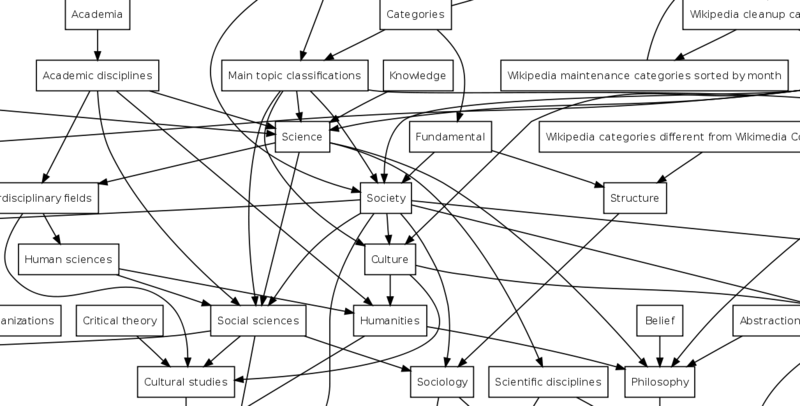
\includegraphics[width=14.155cm,height=7.183cm]{Capitulo2-img4.png}\end{minipage}
\end{center}
{\selectlanguage{spanish}\sffamily
Cualquier categor\'ia puede tener \textit{subcategor\'ias
}(Figura~\ref{seq:refFigura1})\textit{ }y es posible que una
categor\'ia sea subcategor\'ia de m\'as de un \textit{padre} y que
matem\'aticamente, el sistema de categor\'ias se aproxima a un
\textit{grafo ac\'iclico dirigido}\footnote{Wikipedia:Categorization,
\url{http://en.wikipedia.org/wiki/Wikipedia:Categorization}}\textit{:}}


\bigskip

\begin{equation*}
\mathit{Se}\mathit{dice}\mathit{que}A\mathit{es}\mathit{una}\mathit{categor\text{\'i}a}\mathit{padre}\mathit{de}B,\mathit{cuando}B\mathit{es}\mathit{subcategor\text{\'i}a}\mathit{de}\mathit{A.}
\end{equation*}

\bigskip



\begin{center}
\begin{minipage}{10.583cm}
{\centering\selectlanguage{spanish}\itshape
Figura {\refstepcounter{Figura}\theFigura\label{seq:refFigura1}}:
Estructura de categor\'ias y subcategor\'ias.
\par}
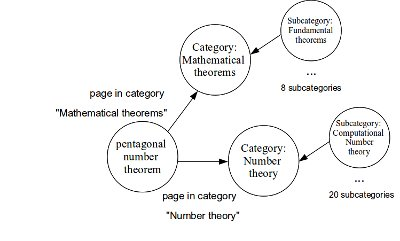
\includegraphics[width=10.583cm,height=6.376cm]{Capitulo2-img5.jpg}\end{minipage}
\end{center}
{\selectlanguage{spanish}\sffamily
Existen gu\'ias del uso recomendado del software de MediaWiki y de
edici\'on de art\'iculos, que sugieren evitar la creaci\'on de ciclos,
sin embargo, debido al volumen de la Wikipedia y la libertad de los
usuarios para elegir libremente los criterios para generar, nombrar los
art\'iculos y clasificarlos (Folksonom\'ia\footnote{Folksonom\'ia es la
traducci\'on al espa\~nol de la palabra folksonomy que surge de la
combinaci\'on de los morfemas en ingl\'es Folk (gente) y taxonomy
(taxonom\'ia), que es el resultado del etiquetado colaborativo,
clasificaci\'on social, clasificaci\'on colectiva o indexado social
para crear y administrar contenidos digitales.}) en las que no se
establecen expl\'icitamente relaciones sem\'anticas subyacentes, la
calidad con la que se organizan los art\'iculos en categor\'ias es
altamente variable, existen algunas muy detalladas y bien organizadas y
en otros casos la categorizaci\'on se ha dado de manera ad hoc o
pobremente.}


\bigskip

{\selectlanguage{spanish}\sffamily
\textstylebibuscitbase{\foreignlanguage{spanish}{Tampoco existe una
restricci\'on sobre el tipo de categor\'ia de mayor nivel al que debe
vincularse una categor\'ia hija, por tanto la estructura de
categor\'ias no se considera estrictamente
como}}\textstylebibuscitbase{\foreignlanguage{spanish}{ un
\'arbol}}\textstylebibuscitbase{\foreignlanguage{spanish}{ o un grafo
ac\'iclico dirigido, ya existen casos parad\'ojicos en los que una
categor\'ia puede ser su propio padre
}}\textstylebibuscitbase{\foreignlanguage{spanish}{(Kittur et al.,
2009)}}\textstylebibuscitbase{\foreignlanguage{spanish}{.}}}


\bigskip

{\selectlanguage{spanish}\sffamily
\textstylebibuscitbase{\foreignlanguage{spanish}{De acuerdo a
}}\textstylebibuscitbase{\foreignlanguage{spanish}{(Zesch \& Gurevych,
2007)}}\textstylebibuscitbase{\foreignlanguage{spanish}{, la
organizaci\'on de las categor\'ias tambi\'en es como un grafo con una
estructura taxon\'omica, en el que cada categor\'ia puede tener un
n\'umero arbitrario de subcategor\'ias en el que se establecen
relaciones de hiponimia o meronimia, y tampoco se considera del todo
estricta, debido a la existencia de ciclos y categor\'ias
disconexas}}\footnote{\textstylebibuscitbase{\foreignlanguage{english}{\textrm{De
acuerdo a los autores, para mayo 15 del 2006, en la Wikipedia en
alem\'an, el componente con m\'as conexiones del grafo de categor\'ias
de Wikipedia contenia 99.8\% de todos los nodos de categor\'ias y 7
ciclos.}}}}\textstylebibuscitbase{\foreignlanguage{spanish}{.}}}


\bigskip

{\selectlanguage{spanish}\sffamily
\textstylebibuscitbase{\foreignlanguage{spanish}{Por otro lado, para
}}\textstylebibuscitbase{\foreignlanguage{spanish}{(Ponzetto \& Strube,
2007b)}}\textstylebibuscitbase{\foreignlanguage{spanish}{ el sistema de
categor\'ias es como un tesauro organizado tem\'aticamente, en el que
las categor\'ias no forman una estructura arb\'orea, sino un grafo
dirigido }}\textstylebibuscitbase{\foreignlanguage{spanish}{(Ponzetto
\& Strube, 2006b)}}\textstylebibuscitbase{\foreignlanguage{spanish}{,
en el que un art\'iculo puede aparecer en m\'as de una categor\'ia, y
cada categor\'ia puede tener m\'as de una categor\'ia padre.}}}


\bigskip

{\selectlanguage{spanish}\sffamily
\textstylebibuscitbase{\foreignlanguage{spanish}{Todas estas
percepciones son coincidentes al mencionar que la estructura de
categor\'ias no puede considerarse de manera incuestionable como un
grafo o una taxonom\'ia, ya que la libertad del ambiente colaborativo
genera que sea desordenada, mal formada y dif\'icil de encontrarle
sentido }}\textstylebibuscitbase{\foreignlanguage{spanish}{(Kittur et
al., 2009)}}\textstylebibuscitbase{\foreignlanguage{spanish}{. De
aqu\'i que para el PLN, su tratamiento sea diverso como se documenta en
el resto del cap\'itulo.}}}


\bigskip


\bigskip

\paragraph[2.2.7 Wikipedia como recurso para
descarga]{\textstylebibuscitbase{\foreignlanguage{spanish}{2.2.7
Wikipedia como recurso para descarga}}}

\bigskip

{\selectlanguage{spanish}\sffamily
\textstylebibuscitbase{\foreignlanguage{spanish}{Al ser un proyecto de
software libre, Wikimedia permite descargar}}\footnote{P\'agina de
informaci\'on de los archivos de descarga de la Wikipedia
\url{http://en.wikipedia.org/wiki/Wikipedia:Database_download}}\textstylebibuscitbase{\foreignlanguage{spanish}{
el contenido wiki de la Wikipedia, en forma de archivos de respaldo
(}}\textstylebibuscitbase{\foreignlanguage{spanish}{\textit{dumps}}}\textstylebibuscitbase{\foreignlanguage{spanish}{),
el sitio de Wikipedia para descarga menciona los posibles usos de este
recurso:}}}


\bigskip

\liststyleLv
\begin{itemize}
\item {\selectlanguage{spanish}\sffamily
\textstylebibuscitbase{\foreignlanguage{spanish}{con prop\'ositos de
respaldos,}}}
\item {\selectlanguage{spanish}\sffamily
\textstylebibuscitbase{\foreignlanguage{spanish}{pasa uso fuera de
l\'inea,}}}
\item {\selectlanguage{spanish}\sffamily
\textstylebibuscitbase{\foreignlanguage{spanish}{con fines
acad\'emicos,}}}
\item {\selectlanguage{spanish}\sffamily
\textstylebibuscitbase{\foreignlanguage{spanish}{para publicar bajo los
t\'erminos de las licencias pertinentes,}}}
\item {\selectlanguage{spanish}\sffamily
\textstylebibuscitbase{\foreignlanguage{spanish}{por diversi\'on.}}}
\end{itemize}

\bigskip

{\selectlanguage{spanish}\sffamily
\textstylebibuscitbase{\foreignlanguage{spanish}{Los archivos para
descarga est\'an protegidos bajo los t\'erminos de las licencias
Creative Commons Attribution-ShareAlike License 3.0 (CC-BY-SA) y GNU
Free Documentation License (GFDL).}}}


\bigskip

{\selectlanguage{spanish}\sffamily
\textstylebibuscitbase{\foreignlanguage{spanish}{Los
}}\textstylebibuscitbase{\foreignlanguage{spanish}{\textit{dumps}}}\textstylebibuscitbase{\foreignlanguage{spanish}{
est\'an en SQL o en XML en el sitio
}}\url{http://dumps.wikimedia.org/}\textstylebibuscitbase{\foreignlanguage{spanish}{.
Las }}\textstylebibuscitbase{\foreignlanguage{spanish}{im\'agenes y
otros archivos con o sin derechos de autor, se descargan por separado
en base a t\'erminos de uso diferentes de los que tienen los archivos
de texto.}}}


\bigskip

\paragraph{2.3 Representaciones de Wikipedia}

\bigskip

{\selectlanguage{spanish}\sffamily
En este sentido, para las tareas de PLN se tiene noci\'on de que la
Wikipedia ha sido considerada como\textstyleFootnoteSymbol{:}}


\bigskip

\liststyleWWviiiNumvii
\begin{itemize}
\item {\selectlanguage{spanish}\sffamily
Corpus, por su una amplia colecci\'on de textos.}
\item {\selectlanguage{spanish}\sffamily
Tesauro, con relaciones jer\'arquicas y de equivalencia entre t\'erminos
y relaciones como la sinonimia, entre otras. }
\item {\selectlanguage{spanish}\sffamily
\textcolor{black}{Base de conocimiento, los art\'iculos en Wikipedia se
encuentran fuertemente interconectados y esta estructura se enriquece
con su sistema de categor\'ias
}\textstylebibuscitbase{\textcolor{black}{(Zesch et al.,
2008a)}}\textcolor{black}{.}}
\item {\selectlanguage{spanish}\sffamily
Base de datos, extracci\'on y codificaci\'on de estructuras y
relaciones.}
\item {\selectlanguage{spanish}\sffamily
Ontolog\'ia, la expresi\'on formal de las relaciones en la Web
Sem\'antica y construcciones l\'ogicas.}
\item {\selectlanguage{spanish}\sffamily
Estructura de red, an\'alisis de las relaciones y extracci\'on, sobre
una representaci\'on tipo grafo de red (network graph).}
\end{itemize}

\bigskip

{\centering\selectlanguage{spanish}\sffamily
FALTA AMPLIAR LA LISTA
\par}

\paragraph{2.4 Wikipedia en el Procesamiento de Lenguaje Natural}

\bigskip

{\selectlanguage{spanish}\sffamily
\textstylebibuscitbase{\foreignlanguage{spanish}{Wikipedia constituye
base amplia de conocimiento l\'exico-sem\'antica, que por sus
caracter\'isticas ha permitido que sea utilizada en el Procesamiento de
Lenguaje Natural en tareas tales como
}}\textstylebibuscitbase{\foreignlanguage{spanish}{(Zesch et al.,
2008a)}}\textstylebibuscitbase{\foreignlanguage{spanish}{:}}}


\bigskip

\liststyleWWviiiNumxi
\begin{itemize}
\item {\selectlanguage{spanish}\sffamily
\textstylebibuscitbase{\foreignlanguage{spanish}{Recuperaci\'on de
informaci\'on,}}}
\item {\selectlanguage{spanish}\sffamily
\textstylebibuscitbase{\foreignlanguage{spanish}{Categorizaci\'on de
textos,}}}
\item {\selectlanguage{spanish}\sffamily
\textstylebibuscitbase{\foreignlanguage{spanish}{Wikificaci\'on de
textos,}}}
\item {\selectlanguage{spanish}\sffamily
\textstylebibuscitbase{\foreignlanguage{spanish}{B\'usqueda de
respuestas,}}}
\item {\selectlanguage{spanish}\sffamily
\textstylebibuscitbase{\foreignlanguage{spanish}{Res\'umenes
autom\'aticos,}}}
\item {\selectlanguage{spanish}\sffamily
\textstylebibuscitbase{\foreignlanguage{spanish}{C\'alculo de proximidad
sem\'antica,}}}
\item {\selectlanguage{spanish}\sffamily
\textstylebibuscitbase{\foreignlanguage{spanish}{Desambiguaci\'on del
sentido de las palabras.}}}
\end{itemize}

\bigskip

{\selectlanguage{spanish}\sffamily
\textstylebibuscitbase{\foreignlanguage{spanish}{Muchas de las
investigaciones al respecto, han sido motivadas para que el PLN apoye
tareas relacionadas a la educaci\'on.}}}


\bigskip

\paragraph{2.4.1 Recuperaci\'on de Informaci\'on (RI)}

\bigskip

{\selectlanguage{spanish}\sffamily
La recuperaci\'on de informaci\'on (RI) debe interpretar los contenidos
de los documentos y hacer un ranking de las respuestas. La consulta no
es estructurada y puede ser ambigua. La relevancia es el principal
punto de inter\'es (Baeza-Yates \& Berthier, 1999).}


\bigskip

{\selectlanguage{spanish}\sffamily
La base documental m\'as grande del mundo, es sin duda la Web, sin
embargo presenta algunos problemas como:}


\bigskip

\liststyleWWviiiNumiv
\begin{itemize}
\item {\selectlanguage{spanish}\sffamily
No hay responsables de todos los contenidos,}
\item {\selectlanguage{spanish}\sffamily
No es f\'acil buscar ni indexar,}
\item {\selectlanguage{spanish}\sffamily
No se usa un lenguaje \'util para las m\'aquinas.}
\end{itemize}

\bigskip

{\selectlanguage{spanish}\sffamily
La RI se basa en la utilizaci\'on de t\'erminos para indexar y recuperar
documentos. Indexar un documento consiste en representar su contenido
por un conjunto de t\'erminos \'indices. Recuperar significa
especificar un conjunto de t\'erminos que deben hallarse entre los
\'indices del documento, estableciendo un ranking de relevancia.}


\bigskip

{\selectlanguage{spanish}\sffamily
El problema de recuperaci\'on de la informaci\'on es la manera de
predecir la relevancia de los documentos y su ranking. Las distintas
premisas utilizadas en el c\'alculo de la relevancia dar\'an lugar a
distintos modelos de trabajo (Figura~\ref{seq:refFigura2}) o de
recuperaci\'on de informaci\'on.}



\begin{center}
\begin{minipage}{13.132cm}
{\centering\selectlanguage{spanish}\itshape
Figura {\refstepcounter{Figura}\theFigura\label{seq:refFigura2}}:
Taxonom\'ia de los Modelos de Recuperaci\'on de Informaci\'on
(Baeza-Yates \& Berthier, 1999).
\par}
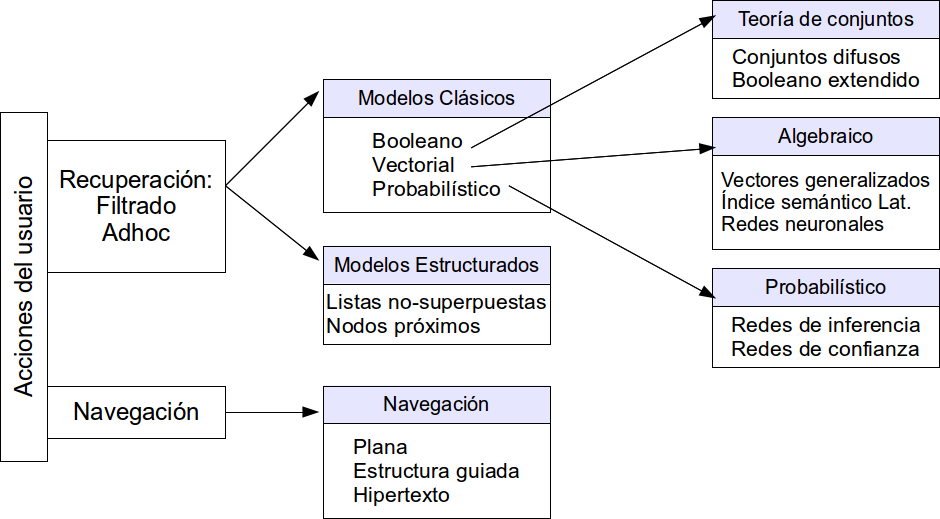
\includegraphics[width=13.132cm,height=7.25cm]{Capitulo2-img6.png}\end{minipage}
\end{center}
{\selectlanguage{spanish}\sffamily
El modelo de la t\'ecnica RI se define como una cu\'adrupla 
$[D,Q,F,R(q_{i},d_{j})]$, con:}


\bigskip

\liststyleWWviiiNumiii
\begin{enumerate}
\item {\selectlanguage{spanish}\sffamily
 $D$ es un conjunto de representaciones de documentos }
\item {\selectlanguage{spanish}\sffamily
 $Q$ es un conjunto de representaciones de necesidades de informaci\'on
de los usuarios}
\item {\selectlanguage{spanish}\sffamily
 $F$ es un marco de modelado de documentos, consultas y sus relaciones}
\item {\selectlanguage{spanish}\sffamily
 $R(q_{i},d_{j})$  es una funci\'on de ranking que asocia un n\'umero
real con una consulta y un documento. El ranking define el orden en el
que el documento satisface la consulta.}
\end{enumerate}

\bigskip

{\selectlanguage{spanish}\sffamily
Las premisas que forman la base para los algoritmos de ranking
determinan el modelo de IR a seguir.}


\bigskip

\paragraph{2.5 Categorizaci\'on de textos}

\bigskip

{\selectlanguage{spanish}\sffamily
La categorizaci\'on de textos consiste en asignar documentos a dos o
m\'as subcategor\'ias, que ya han sido definidas como resultado de
procesos de Recuperaci\'on de Informaci\'on al entrenar corpus de
documentos que previamente fueron clasificados. (Manning \& Hinrich,
1999).}


\bigskip

{\selectlanguage{spanish}\sffamily
Mayormente, los clasificadores de texto utilizan t\'ecnicas de
aprendizaje de m\'aquina y representan los textos como \textit{bag of
words (BOW).}}


\bigskip

{\selectlanguage{spanish}\sffamily
La informaci\'on contenida en Wikipedia, ha sido utilizada tambi\'en
para crear un clasificador auxiliar de texto, que permite relacionar
documentos con art\'iculos relevantes de Wikipedia, esto es, con los
conceptos de los art\'iculos se aumenta espacio de palabras (o BOW),
m\'etodo que los autores enmarcan en el constructivismo
inductivo\footnote{Estudio de m\'etodos que dotan al estudiante con la
habilidad de modificar o mejorar la representaci\'on del lenguaje.}
(Gabrilovich \& Evgeniy, 2006).}


\bigskip

{\selectlanguage{spanish}\sffamily
El procesamiento utiliza texto plano, que permite aplicar los algoritmos
de similitud para identificar autom\'aticamente los art\'iculos
relevantes para cada documento. Se realiza un generador de
caracter\'isticas, que trabaja en cada documento con contextos
individuales de diferentes niveles: por palabras , sentencias,
despu\'es p\'arrafos y finalmente con el documento completo. Al
trabajar con contextos individuales, impl\'icitamente se realiza
desambiguaci\'on del sentido de las palabras y se controla la
polisemia, gracias al contexto y texto \ circundante.}


\bigskip

{\selectlanguage{spanish}\sffamily
En este caso, de acuerdo a lo expuesto por los autores, si se quiere
informaci\'on sobre {\textquotedblleft}jaguar car
models{\textquotedblright} los resultados tendr\'an \'unicamente
relaci\'on con autos y modelos de autos, mientras que si se solicita
informaci\'on de {\textquotedblleft}jaguar Panthera
onca{\textquotedblright} los resultados ser\'an relacionados a
animales.}


\bigskip


\bigskip

\subsubsection[Grafos de Wikipedia]{Grafos de Wikipedia}
\hypertarget{RefHeading333457232820}{}
\bigskip

{\selectlanguage{spanish}\sffamily
Como se ha mencionado, Wikipedia tiene una estructura organizada, que
puede apreciarse en sus categor\'ias y los v\'inculos entre
art\'iculos. Otra forma de organizaci\'on en la que es concebida la
Wikipedia es como un grafo dirigido, en el que los nodos son temas y
las aristas son los hiperv\'inculos entre estos. Este tipo de
estructura comparte caracter\'isticas topol\'ogicas similares a las de
la WWW (World Wide Web) \textstylebibuscitbase{(Capocci2006)},}


\bigskip

{\selectlanguage{spanish}\sffamily
Suponiendo que cada art\'iculo de Wikipedia puede vincularse a un
n\'umero arbitrario de categor\'ias, en la que cada categor\'ia es un
tipo de etiqueta sem\'antica para ese art\'iculo. Una categor\'ia
regresa los v\'inculos, a todos los art\'iculos de esa categor\'ia,
adem\'as de visualizarse como un solo grafo, se le ha tratado como
grafos espec\'ificos: }

\liststyleLvi
\begin{itemize}
\item {\selectlanguage{spanish}\sffamily
el \textit{grafo de categor\'ias
}\foreignlanguage{spanish}{\textit{GCW}}\textit{ (Wikipedia Category
Graph)} y }
\item {\selectlanguage{spanish}\sffamily
el \textit{grafo de art\'iculos GAW \ (Wikipedia Article Graph)}.}
\end{itemize}

\bigskip

{\selectlanguage{spanish}\sffamily
Los grafos de art\'iculos y categor\'ias est\'an fuertemente vinculados
(Figura \ref{seq:refFigura3}) pero son tratados como estructuras
diferentes, cada una con sus propias caracter\'isticas espec\'ificas.}


\bigskip



\begin{center}
\begin{minipage}{11.015cm}
{\centering\selectlanguage{spanish}\itshape
Figura {\refstepcounter{Figura}\theFigura\label{seq:refFigura3}}:
Relaci\'on entre los grafos de categor\'ias (GCW) y de art\'iculos
(GAW) de Wikipedia.
\par}
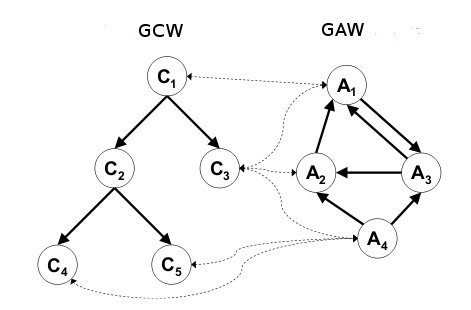
\includegraphics[width=11.015cm,height=6.899cm]{Capitulo2-img7.jpg}\end{minipage}
\end{center}
{\selectlanguage{spanish}\sffamily
Esta separaci\'on obedece a que, los v\'inculos entre art\'iculos son
las relaciones producto del trabajo colaborativo, mientras que los
v\'inculos entre categor\'ias son establecidos por relaciones de
hiponimia o meronimia\textstylebibuscitbase{
}\textstylebibuscitbase{(18)}. }


\bigskip

{\selectlanguage{spanish}\sffamily
En el PLN, Wikipedia en su forma de grafo, mayormente como GCW, ha sido
explotado como:}


\bigskip

\liststyleLvii
\begin{itemize}
\item {\selectlanguage{spanish}\sffamily
\foreignlanguage{spanish}{Mapa de categor\'ias basado en la
co-ocurrencia de categor\'ias
}\textstylebibuscitbase{\foreignlanguage{spanish}{(Holloway)}}\textstylebibuscitbase{\foreignlanguage{spanish}{.}}}
\item {\selectlanguage{spanish}\sffamily
\textstylebibuscitbase{\foreignlanguage{spanish}{Tesauro que combina
etiquetado colaborativo e indexado jer\'arquico
}}\textstylebibuscitbase{\foreignlanguage{spanish}{(Voss2006)}}\textstylebibuscitbase{\foreignlanguage{spanish}{.}}}
\item {\selectlanguage{spanish}\sffamily
\textstylebibuscitbase{\foreignlanguage{spanish}{Fuente de conocimiento
l\'exico-sem\'antica
}}\textstylebibuscitbase{\foreignlanguage{spanish}{(Zesch2007)}}\textstylebibuscitbase{\foreignlanguage{spanish}{.}}}
\end{itemize}

\bigskip

\subsubsection[Grafo de categor\'ias de Wikipedia {}-GCW]{Grafo de
categor\'ias de Wikipedia -GCW}
\hypertarget{RefHeading10776782078703}{}
\bigskip

{\selectlanguage{spanish}\sffamily
El grafo de categor\'ias de Wikipedia - GCW es equiparable a los grafos
bien tipificados de las redes l\'exico-sem\'anticas. Es el resultado
del ambiente colaborativo en el que se ha construido Wikipedia.}


\bigskip

{\selectlanguage{spanish}\sffamily
Como se ha mencionado el GCW tiene caracter\'isticas y propiedades de
las redes l\'exico-sem\'anticas, como WordNet y ha sido utilizado como
un recurso en el PLN, por ejemplo, para calcular la proximidad
sem\'antica
\textstylebibuscitbase{(Zesch2007)}\textstylebibuscitbase{.}}


\bigskip

{\selectlanguage{spanish}\sffamily
Para el c\'alculo de proximidad sem\'antica del GCW se ha probado por
medio de un an\'alisis formal, basado en la teor\'ia de grafos y
orientado particularmente para redes sem\'anticas de palabras
(wordnets).}


\bigskip

{\selectlanguage{spanish}\sffamily
\textstylebibuscitbase{Para este an\'alisis el grafo dirigido de
categor\'ias } $G$\textstylebibuscitbase{, se trata como un
}\textstylebibuscitbase{grafo no dirigido,}\textstylebibuscitbase{ dado
que las relaciones que conectan categor\'ias son reversibles:}}

{\centering\selectlanguage{spanish}
\textstylebibuscitbase{Learning to link with Wikipedia.} $G=(V,E)$
\par}

{\selectlanguage{spanish}\sffamily
\textstylebibuscitbase{donde, }}

{\selectlanguage{spanish}\sffamily
 $V$ \textstylebibuscitbase{ representa el conjunto de nodos o
v\'ertices y}}

{\selectlanguage{spanish}\sffamily
 $E$ \textstylebibuscitbase{es el conjunto no ordenado de pares de
distintos v\'ertices, conocidos como arcos o
}\textstylebibuscitbase{aristas}\textstylebibuscitbase{.}}


\bigskip

{\selectlanguage{spanish}\sffamily
\textstylebibuscitbase{Cada p\'agina se considera un
}\textstylebibuscitbase{\textit{nodo}} $n$ \textstylebibuscitbase{ ,
cada v\'inculo entre p\'aginas es un arco o }\textstylebibuscitbase{una
}\textstylebibuscitbase{arista } $e$ \textstylebibuscitbase{\textit{.
}}\textstylebibuscitbase{C\'omo los grafos de estructuras sem\'anticas,
el GCW se puede }\textstylebibuscitbase{definir por el conjunto de
par\'ametros propios de los grafos, como lo son: }}


\bigskip

\liststyleLviii
\begin{itemize}
\item {\selectlanguage{spanish}\sffamily
\textstylebibuscitbase{\textit{grado de los nodos }} $k$
\textstylebibuscitbase{, que es el n\'umero de arcos conectados con ese
}\textstylebibuscitbase{nodo.}}
\item {\selectlanguage{spanish}\sffamily
\textstylebibuscitbase{\textit{grado promedio }} $\bar{k}$
\textstylebibuscitbase{, el promedio sobre todos los nodos.}}
\item {\selectlanguage{spanish}\sffamily
\textstylebibuscitbase{\textit{rutas o caminos entre
nodos}}\textstylebibuscitbase{ } $p_{i,j}$ \textstylebibuscitbase{, es
la secuencia de los arcos que conectan a }\textstylebibuscitbase{un
nodo } $n_{i}$ \textstylebibuscitbase{con un nodo } $n_{j}$
\textstylebibuscitbase{.}}
\item {\selectlanguage{spanish}\sffamily
\textstylebibuscitbase{\textit{longitud de ruta}}\textstylebibuscitbase{
} $l(p_{i,j})$ \textstylebibuscitbase{, es el n\'umero de arcos en la
ruta. Puede haber }\textstylebibuscitbase{m\'as de una ruta entre los
nodos, de modo que se puede calcular la longitud de la ruta m\'as corta
} $L_{i},j=\mathit{min}l(p_{i,j})$ \textstylebibuscitbase{.}}
\item {\selectlanguage{spanish}\sffamily
\textstylebibuscitbase{\textit{promedio de la ruta m\'as
corta}}\textstylebibuscitbase{ } $\bar{L}$ \textstylebibuscitbase{sobre
todos los nodos. }}
\item {\selectlanguage{spanish}\sffamily
\textstylebibuscitbase{\textit{di\'ametro }} $D$
\textstylebibuscitbase{\textit{, }}\textstylebibuscitbase{es la
m\'axima longitud de la ruta m\'as corta entre todos los
}\textstylebibuscitbase{pares de nodos del grafo.}}
\item {\selectlanguage{spanish}\sffamily
\textstylebibuscitbase{\textit{coeficiente de
cluster}}\textstylebibuscitbase{ de un nodo } $n_{i}$
\textstylebibuscitbase{puede calcularse de la siguiente manera:}}
\end{itemize}
\begin{equation*}
C_{i}=\frac{T_{i}}{\frac{k_{i}(k_{i}-1)}{2}}=\frac{2T_{i}}{k_{i}(k_{i}-1)}
\end{equation*}
{\selectlanguage{spanish}\sffamily
\textstylebibuscitbase{donde } $T_{i}$ \textstylebibuscitbase{se refiere
al n\'umero de arcos entre vecinos del nodo } $n_{i}$
\textstylebibuscitbase{y } $k_{i}(k_{i}-1)/{2}$
\textstylebibuscitbase{es el n\'umero m\'aximo de arcos que pueden
existir entre los } $k_{i}$ \textstylebibuscitbase{vecinos del nodo }
$n_{i}$ \textstylebibuscitbase{.}}

{\selectlanguage{spanish}\sffamily
\textstylebibuscitbase{El coeficiente de cluster } $C$
\textstylebibuscitbase{para todo el grafo es el promedio de todos los }
$C_{i}$ \textstylebibuscitbase{. En un grafo conexo, el coeficiente de
cluster es 1.}}


\bigskip

{\selectlanguage{spanish}\sffamily
\textstylebibuscitbase{Las medidas de proximidad sem\'antica aplicables
a redes sem\'anticas de palabras (i.e. WordNet, tesauro Roget, entre
otras }\textstylebibuscitbase{(Zesch2007)}\textstylebibuscitbase{) se
aplican sobre el GCW:}}


\bigskip

\liststyleLix
\begin{itemize}
\item {\selectlanguage{spanish}\sffamily
\textstylebibuscitbase{Todos los grafos analizados son grafos de mundos
peque\~nos}%
%small world graphs DEFINIR
\textstylebibuscitbase{, los cuales contienen clusters que est\'an
conectados por v\'inculos de rangos amplios que conducen a valores
peque\~nos de } $\bar{L}$ \textstylebibuscitbase{y } $D$
\textstylebibuscitbase{, esto es, los grafos de mundos peque\~nos
est\'an caracterizados por tener (i) valores peque\~nos de } $\bar{L}$
\textstylebibuscitbase{y (ii) valores altos de } $C$
\textstylebibuscitbase{.}}
\item {\selectlanguage{spanish}\sffamily
\textstylebibuscitbase{Todas las redes sem\'anticas son grafos de escala
libre (scale-free graphs), ya que su grado de distribuci\'on sigue una
ley exponencial.}}
\end{itemize}

\bigskip

{\selectlanguage{spanish}\sffamily
\textstylebibuscitbase{De modo particular los resultados demostraron que
tanto WordNet como el }\textstylebibuscitbase{GCW son (i) grafos de
libre escala y grafos de mundos peque\~nos y (ii) tienen un conjunto de
par\'ametros muy similar.}}


\bigskip

\subsubsection[Medidas de proximidad sem\'antica aplicadas a un
grafo]{Medidas de proximidad sem\'antica aplicadas a un grafo}
\hypertarget{RefHeading10778782078703}{}
\bigskip

{\selectlanguage{spanish}\sffamily
Existen muchas medidas para el c\'alculo de proximidad sem\'antica en
redes sem\'anticas
\textstylebibuscitbase{(Zesch2007)}\textstylebibuscitbase{ (Tabla 2)}:}


\bigskip

{\centering\selectlanguage{spanish}\sffamily\itshape
Tabla 2. Medidas basadas en WordNet y aplicables a Wikipedia
\par}

\begin{flushleft}
\tablehead{}
\begin{supertabular}{|m{2.261cm}|m{5.039cm}|m{7.9190006cm}|}
\hline
\centering \selectlanguage{spanish}\bfseries Autor &
\centering \selectlanguage{spanish}\bfseries Descripci\'on &
\centering\arraybslash \selectlanguage{spanish}\bfseries
C\'alculo\\\hline
{\selectlanguage{spanish} Rada et al.}

\selectlanguage{spanish} (1989) &
\selectlanguage{spanish} Longitud de la ruta en arcos (Path Lenght)
entre dos nodos.  &
\begin{equation*}
\mathit{dist}_{\mathit{PL}}=l(n_{1},n_{2})
\end{equation*}
\\\hline
{\selectlanguage{spanish} Leacock y Chodorow}

\selectlanguage{spanish} (1998) &
\selectlanguage{spanish} Normaliza la longitud de la ruta con la
profundidad del grafo &
\begin{equation*}
\text{sim}_{\mathit{LC}}(n_{1},n_{2})=-\log
(\frac{l(n_{1}),n_{2}}{2\times \mathit{depth}})
\end{equation*}
\\\hline
{\selectlanguage{spanish} Wu y Palmer }

\selectlanguage{spanish} (1994) &
\selectlanguage{spanish} Introduce una medida para saber que tan
similares son los sentidos de dos palabras basandose en la profundidad
de los dos sentidos en la taxonom\'ia y en el Least Common Subsumer de
dos nodos \ (nodo antecesor m\'as espec\'ifico). &
\begin{equation*}
\text{sim}_{\text{WP}}=\frac{2\mathit{depth}(\mathit{lcs})}{l(n_{1},\mathit{lcs})+l(n_{2},\mathit{lcs})+2\mathit{depth}(\mathit{lcs})}
\end{equation*}
\\\hline
{\selectlanguage{spanish} Resnik}

\selectlanguage{spanish} (1995) &
\selectlanguage{spanish} Define la similitud sem\'antica entre dos nodos
como el valor de contenidos de informaci\'on  $(\mathit{IC})$ de su 
$\mathit{lcs}$. Utiliza la frecuencia relativa en un corpus para
estimar el valor de contenido de la informaci\'on. &
\begin{equation*}
\mathit{Res}
\end{equation*}
\\\hline
{\selectlanguage{spanish} Jiang y Conrath}

\selectlanguage{spanish} (1997) &
\selectlanguage{spanish} Adicionalmente usa el IC de los nodos. El
resultado que devuelve es una distancia en lugar de un valor de
similitud. &
\begin{equation*}
\mathit{dist}_{\mathit{JC}}(n_{1},n_{2})=\mathit{IC}(n_{1})+\mathit{IC}(n_{2})-2\mathit{IC}(\mathit{lcs})
\end{equation*}
\\\hline
{\selectlanguage{spanish} Lin}

\selectlanguage{spanish} (1998) &
\selectlanguage{spanish} Define la similitud sem\'antica usando una
formula derivada de la teor\'ia de la informaci\'on. &
\begin{equation*}
\text{sim}_{\mathit{Lin}}(n_{1},n_{2})=\frac{2\times
{\mathit{IC}(\mathit{lcs})}}{\mathit{IC}(n_{1})+\mathit{IC}(n_{2})}
\end{equation*}
\\\hline
\end{supertabular}
\end{flushleft}

\bigskip

{\selectlanguage{spanish}\sffamily
Como las palabras polis\'emicas pueden tener m\'as de un nodo
correspondiente en una red sem\'antica de palabras, la proximidad
sem\'antica entre dos palabras  $w_{1}$ y  $w_{2}$ puede calcularse de
la siguiente manera:}


\bigskip



\begin{center}
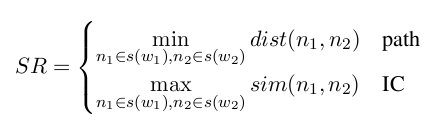
\includegraphics[width=8.483cm,height=2.429cm]{Capitulo2-img8.jpg}
\end{center}
{\selectlanguage{spanish}\sffamily
donde  $s(w_{i})$ es el conjunto de nodos que representa sentidos de la
palabra  $w_{i}$, esto significa, que la proximidad de dos palabras es
igual al par de nodos m\'as relacionados.}


\bigskip

{\selectlanguage{spanish}\sffamily
\textstylebibuscitbase{\foreignlanguage{spanish}{A diferencia de otras
redes l\'exico-sem\'anticas, los nodos del GCW no son synsets o
t\'erminos \'unicos, sino un concepto generalizado o una categor\'ia,
de }}\textstylebibuscitbase{\foreignlanguage{spanish}{modo que es
necesario hacer modificaciones para adaptar las medidas de
}}\textstylebibuscitbase{\foreignlanguage{spanish}{proximidad
sem\'antica al GCW. La proximidad sem\'antica entre art\'iculos se mide
}}\textstylebibuscitbase{\foreignlanguage{spanish}{por las categor\'ias
asignadas a los art\'iculos.}}}


\bigskip

{\selectlanguage{spanish}\sffamily
\textstylebibuscitbase{\foreignlanguage{spanish}{Se definen }} $C_{1}$
\textstylebibuscitbase{\foreignlanguage{spanish}{y }} $C_{2}$
\textstylebibuscitbase{\foreignlanguage{spanish}{como un conjunto de
categor\'ias asignadas a los
}}\textstylebibuscitbase{\foreignlanguage{spanish}{art\'iculos }}
$a_{i}$ \textstylebibuscitbase{\foreignlanguage{spanish}{ y }} $a_{j}$
\textstylebibuscitbase{\foreignlanguage{spanish}{ respectivamente. Se
determina la proximidad sem\'antica para cada par de categor\'ias }}
$(c_{k},c_{l})$ \textstylebibuscitbase{\foreignlanguage{spanish}{ con
}} $c_{k}{\in}C_{1}$ \textstylebibuscitbase{\foreignlanguage{spanish}{y
}} $c_{l}{\in}C_{2}$ \textstylebibuscitbase{\foreignlanguage{spanish}{.
Se selecciona el valor m\'as apropiado de entre todos los pares }}
$(c_{k},c_{l})$ \textstylebibuscitbase{\foreignlanguage{spanish}{, como
por ejemplo, el valor m\'inimo para basados en ruta y el m\'aximo para
las medidas basadas en
}}\textstylebibuscitbase{\foreignlanguage{spanish}{contenidos de
informaci\'on.}}}



\begin{center}
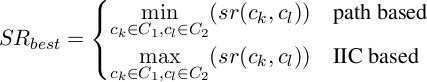
\includegraphics[width=9.059cm,height=1.741cm]{Capitulo2-img9.jpg}
\end{center}
{\selectlanguage{spanish}\sffamily
\textstylebibuscitbase{\foreignlanguage{spanish}{Si se sustituye el
contenido de informaci\'on de Resnik con informaci\'on de contenido
intr\'inseco IIC del grafo subyacente se obtienen mejores resultados y
adem\'as es independiente de corpus, el IIC de un nodo }} $n_{i}$
\textstylebibuscitbase{\foreignlanguage{spanish}{:}}}



\begin{center}
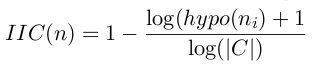
\includegraphics[width=6.652cm,height=1.466cm]{Capitulo2-img10.jpg}
\end{center}
{\selectlanguage{spanish}\sffamily
donde:}

{\selectlanguage{spanish}\sffamily
\ \  $\mathit{hypo}(n_{i})$ es el n\'umero de hip\'onimos de  $n_{i}$ y}

{\selectlanguage{spanish}\sffamily
\ \  $|C|$ es el n\'umero de nodos de la taxonom\'ia.}


\bigskip

{\selectlanguage{spanish}\sffamily
Para contar adecuadamente el n\'umero de hip\'onimos se debe de romper
ciclos del GCW pero sin desconectar nodos de un componente conexo.%
%Este p\'arrafo esta incorrecto e incompleto. Revisar de Analysis of WCG
}


\bigskip

{\selectlanguage{spanish}\sffamily
Una vez que se realizaron los c\'alculos y adecuaciones correspondientes
de acuerdo a la informaci\'on que se ha descrito, los resultados se
comparan con un est\'andar de oro, en este caso con tres conjuntos de
datos en idioma alem\'an y posteriormente con el momento de producto de
correlaci\'on de Pearson \textit{r }para comparar con las valoraciones
que se hacen de manera manual. Los resultados obtenidos demuestran que
las medidas de proximidad sem\'antica fueron exitosas al ser aplicadas
al GCW.}


\bigskip

\subsubsection[Grafo de art\'iculos de Wikipedia {}-- GAW (Wikipedia
Article Graph)]{Grafo de art\'iculos de Wikipedia -- GAW (Wikipedia
Article Graph)}
\hypertarget{RefHeading10780782078703}{}
\bigskip

{\selectlanguage{spanish}\sffamily
En Wikipedia los art\'iculos est\'an estrechamente relacionados por
medio de la estructura de v\'inculos, dado que los v\'inculos pueden
ser insertado mientras se edita un art\'iculo. El grafo de art\'iculos
se concibe como un grafo dirigido, como el que se muestra en la parte
derecha de la Figura \ref{seq:refFigura3}. Cada art\'iculo es un nodo y
cada v\'inculo entre art\'iculos un arco que va de un nodo hacia otro
\textstylebibuscitbase{(Zesch2007)}. Los v\'inculos entre art\'iculos
se establecen con cualquier tipo de relaci\'on entre estos.}


\bigskip

{\selectlanguage{spanish}\sffamily
Los hiperv\'inculos que apuntan de un art\'iculo hacia otro pueden ser
tratados como v\'inculos dirigidos, mientras que los art\'iculos
representan los nodos de una red
\textstylebibuscitbase{(Zlatic2006)}\textstylebibuscitbase{, un grafo
resultado de la estructura hiper vinculada de los art\'iculos de
Wikipedia }\textstylebibuscitbase{(Buriol2006)}\textstylebibuscitbase{
que es un tipo de grafo de Web. }}


\bigskip

{\selectlanguage{spanish}\sffamily
Los grafos de Web se han estudiado en base a sus propiedades
topol\'ogicas. El estado del arte respecto al GAW parece indicar que se
ha realizado poca investigaci\'on sobre su evoluci\'on estad\'istica y
propiedades topol\'ogicas. Justamente es esta una de las
caracter\'isticas que representa un \'area de oportunidad para el
presente trabajo de tesis.}

%
%pendiente de complementar Buriol et al. Zlatic et al. 


\subsubsection[Relaciones entre palabras]{Relaciones entre palabras}
\hypertarget{RefHeading334457232820}{}
\bigskip

{\selectlanguage{spanish}\sffamily
Una manera de entender los recursos l\'exico-sem\'anticos es estudiar
como se relacionan los significados de las palabras. Las palabras
pueden organizarse en una jer\'arqu\'ia l\'exica, como en el caso de
WordNet, en la que las palabras se organizan jer\'arquicamente. Cada
nodo consiste de un synset de palabras con id\'enticos (o casi
id\'enticos) significados \textstylebibuscitbase{(ManningFoundations)}.
Existen adem\'as otro tipo de relaciones entre palabras como la
meronimia o relaciones \textit{parte-todo, }en la Figura
\ref{seq:refFigura4} se pueden ver otro tipo de estas relaciones.}


\bigskip

{\selectlanguage{spanish}\sffamily
La hiponimia y hiperonimia%
%Descripci\'on breve de \ sinonimia, antonimia, etc
 son tambi\'en relaciones entre palabras. La hiperonima es una palabra
con un sentido m\'as general. La hiponima es una palabra con un
significado m\'as especializado. En general, si w\textsubscript{1} es
una hiperonima de w\textsubscript{2}, entonces
w\foreignlanguage{spanish}{\textsubscript{2}} es un hiponima de
w\foreignlanguage{spanish}{\textsubscript{1.}}}


\bigskip



\begin{center}
\begin{minipage}{15.221cm}
{\centering\selectlanguage{spanish}\itshape
Figura {\refstepcounter{Figura}\theFigura\label{seq:refFigura4}}:
Relaciones entre palabras.
\par}
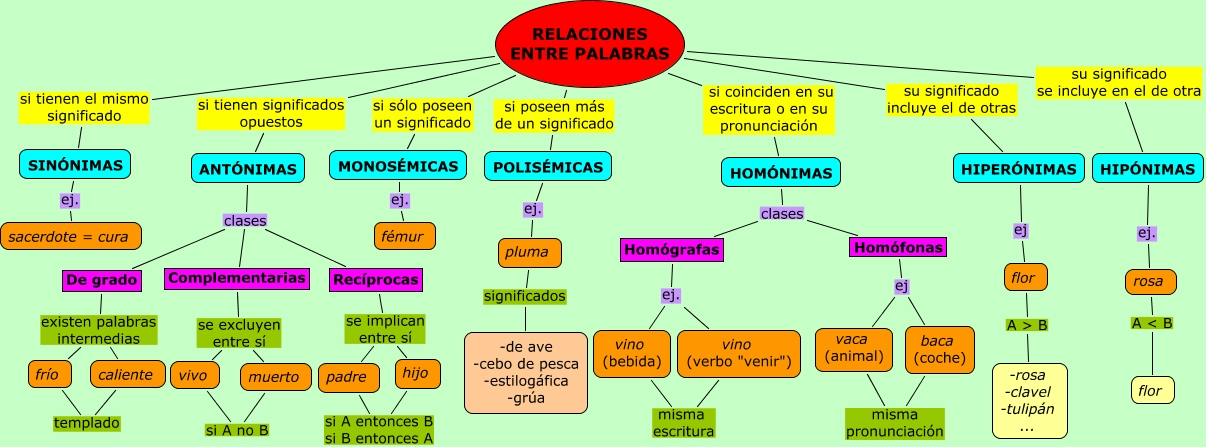
\includegraphics[width=16.591cm,height=6.149cm]{Capitulo2-img11.jpg}\end{minipage}
\end{center}
\subsubsection[WordNet]{WordNet}
\hypertarget{RefHeading334657232820}{}
\bigskip

{\selectlanguage{spanish}\sffamily
WordNet es un sistema de referencia l\'exica, en forma de diccionario
electr\'onico en ingl\'es que fue desarrollado en la universidad de
Princeton. Este recurso combina muchas caracter\'isticas usadas para
desambiguaci\'on del sentido de las palabras en un solo sistema. }


\bigskip

{\selectlanguage{spanish}\sffamily
WordNet, incluye definiciones de sentidos de palabras como un
diccionario, define synsets o conjuntos de sin\'onimos, los cuales
representan un concepto l\'exico, y adem\'as proporciona las relaciones
jer\'arquicas existentes entre palabras. }


\bigskip

{\selectlanguage{spanish}\sffamily
Los sentidos de WordNet comprenden un conjunto de sin\'onimos y
definiciones al igual que un diccionario, las cuales son llamadas
glosas. El n\'umero que se encuentra al inicio de la definici\'on de
algunos sentidos, es la frecuencia de los valores obtenidos del corpus
SemCor. A diferencia de un diccionario, WordNet contiene un conjunto de
relaciones l\'exicas entre sysnsets o lemas, los cuales aparecen al
inicio de la glosa \textstylebibuscitbase{(Torres\_Ramos2009)}.}


\bigskip

{\selectlanguage{spanish}\sffamily
WordNet puede descargarse libremente de Internet y ha sido ampliamente
utilizada en aplicaciones de PLN.}


\bigskip

\subsubsection[Wikipedia como red]{Wikipedia como red}
\hypertarget{RefHeading10782782078703}{}
\bigskip

{\selectlanguage{spanish}\sffamily
Wikipedia comparte caracter\'isticas de las redes l\'exico-sem\'anticas,
las cuales estructuran el vocabulario en funci\'on de las relaciones
sem\'anticas entre palabras, como sinonimia, antonimia, hiponimia,
hiperonimia o meronimia (ie. WordNet)\footnote{Tecnolog\'ias
ling\"u\'isticas: los recursos ling\"u\'isticos
\url{http://liceu.uab.cat/~joaquim/language_technology/HLT/tecnol_ling_recursos.html}.}.}


\bigskip

{\selectlanguage{spanish}\sffamily
\textstylebibuscitbase{Cada Wikipedia (por cada idioma se le considera
una diferente Wikipedia) puede considerarse como una red en la que los
art\'iculos son los nodos y los hiperv\'inculos entre
art\'icu}\textstylebibuscitbase{los son enlaces directos entre ellos
}\textstylebibuscitbase{(Zlatic2006)}\textstylebibuscitbase{.}}


\bigskip


\bigskip


\bigskip

{\selectlanguage{spanish}\sffamily
Ambig\"uedad}


\bigskip

{\selectlanguage{spanish}\sffamily
Una de las tareas del PLN es la resoluci\'on de la ambig\"uedad sobre
como deben ser interpretadas las palabras, esto debido a que una
palabra puede tener m\'as de un significado o sentido (polisemia). }


\bigskip

{\selectlanguage{spanish}\sffamily
La ambig\"uedad, en el proceso ling\"u\'istico, se presenta cuando
pueden admitirse distintas interpretaciones a partir de una
representaci\'on dada o cuando existe confusi\'on al tener diversas
estructuras y no tener los elementos necesarios para eliminar las
eventualmente incorrectas \textstylebibuscitbase{(Torres\_Ramos2006)}.
\foreignlanguage{spanish}{Para desambiguar, es decir, para seleccionar
los significados o
}\textstylebibuscitbase{\foreignlanguage{spanish}{las estructuras m\'as
adecuados de un conjunto distinto de posibilidades, se requieren de
diversas estrategias de soluci\'on en cada caso
}}\textstylebibuscitbase{\foreignlanguage{spanish}{(Galicia\_Haro2007)}}\textstylebibuscitbase{\foreignlanguage{spanish}{.}}}


\bigskip

{\selectlanguage{spanish}\sffamily
\textstylebibuscitbase{\foreignlanguage{spanish}{Se distinguen tres
tipos principales de ambig\"uedad: l\'exica, sem\'antica y sint\'actica
o estructural. }}}


\bigskip

\liststyleLx
\begin{itemize}
\item {\selectlanguage{spanish}\sffamily
\textstylebibuscitbase{\foreignlanguage{spanish}{\textit{Ambig\"uedad
l\'exica}}}\textstylebibuscitbase{\foreignlanguage{spanish}{. Se
presenta cuando las palabras pueden pertenecer
}}\textstylebibuscitbase{\foreignlanguage{spanish}{a diferentes
categor\'ias gramaticales, por ejemplo
}}\textstylebibuscitbase{\foreignlanguage{spanish}{\textit{bajo}}}\textstylebibuscitbase{\foreignlanguage{spanish}{
puede ser una preposici\'on, un sustantivo, un adjetivo o una
conjugaci\'on del verbo bajar. }}}
\item {\selectlanguage{spanish}\sffamily
\textstylebibuscitbase{\foreignlanguage{spanish}{\textit{Ambig\"uedad
sem\'antica}}}\textstylebibuscitbase{\foreignlanguage{spanish}{. Se
presenta cuando las palabras tienen m\'ultiples significados, por
ejemplo la palabra
}}\textstylebibuscitbase{\foreignlanguage{spanish}{\textit{banco}}}\textstylebibuscitbase{\foreignlanguage{spanish}{
puede significar banco de peces, banco para tomar asiento o
instituci\'on financiera. }}}
\item {\selectlanguage{spanish}\sffamily
\textstylebibuscitbase{\foreignlanguage{spanish}{A}}\textstylebibuscitbase{\foreignlanguage{spanish}{\textit{mbig\"uedad
sint\'actica.}}}\textstylebibuscitbase{\foreignlanguage{spanish}{
Tambi\'en conocida como ambig\"uedad estructural se presenta cuando una
oraci\'on puede tener m\'as de una estructura
}}\textstylebibuscitbase{\foreignlanguage{spanish}{sint\'actica. Por
ejemplo, hablando de una pintura de arte en la oraci\'on
}}\textstylebibuscitbase{\foreignlanguage{spanish}{{\textquotedblleft}Este
trabajo no tiene t\'itulo{\textquotedblright}
}}\textstylebibuscitbase{\foreignlanguage{spanish}{(ManningFoundations)}}\textstylebibuscitbase{\foreignlanguage{spanish}{
se pueden entender dos cosas diferentes: a) el trabajo no recibi\'o por
parte de su autor un nombre con el cu\'al pueda denotarse, o bien, b)
la pintura no tiene una placa en la cu\'al pueda leerse el t\'itulo de
la obra.}}}


\bigskip
\end{itemize}
\subsubsection[Desambiguaci\'on del sentido de las
palabras]{Desambiguaci\'on del sentido de las palabras}
\hypertarget{RefHeading10784782078703}{}
\bigskip

{\selectlanguage{spanish}\sffamily
La desambiguaci\'on del sentido de las palabras es una fase necesaria
para la consecuci\'on de tareas de PLN como lo son el an\'alisis
sint\'actico o la interpretaci\'on sem\'antica. La desambiguaci\'on
consiste en asignar autom\'aticamente el sentido adecuado de una
palabra en polis\'emica en un texto con relaci\'on al contexto en el
que se utiliza, las palabras tienen un n\'umero finito discreto de
sentidos, normalmente escritos en un diccionario, tesauro u alguna otra
fuente de referencia
\textstylebibuscitbase{(ManningFoundations)}\textstylebibuscitbase{
}\textstylebibuscitbase{(Mihalcea2007)}.}

{\selectlanguage{spanish}\sffamily
La desambiguaci\'on es considerada una tarea de clasificaci\'on: los
sentidos de la palabra son las clases, el contexto provee la evidencia
y cada ocurrencia de una palabra es asignada a una o m\'as de las
posibles clases en base a la evidencia. \foreignlanguage{spanish}{Si
las decisiones de un sistema }\foreignlanguage{spanish}{dependen del
significado del texto, entonces la desambiguaci\'on es necesaria.}}

{\selectlanguage{spanish}\sffamily
En un sistema de recuperaci\'on de informaci\'on, cuando se realiza una
consulta (query) sobre la palabra \textit{car\'acter }deber\'a devolver
como resultado documentos que traten sobre alguna de las acepciones de
esta palabra, como pueden ser:}


\bigskip

\liststyleLxi
\begin{itemize}
\item {\selectlanguage{spanish}
Se\~nal o marca que se imprime, pinta o esculpe en algo.}
\item {\selectlanguage{spanish}
Conjunto de cualidades o circunstancias propias de una cosa, de una
persona o de una colectividad, que las distingue, por su modo de ser u
obrar, de las dem\'as. \textit{El }\textit{car\'acter espa\~nol.}
\textit{El car\'acter insufrible de Fulano.}}
\item {\selectlanguage{spanish}
Condici\'on dada a alguien o a algo por la dignidad que sustenta o la
funci\'on que desempe\~na. \textit{El car\'acter de juez, de padre.}
\textit{Medidas de car\'acter transitorio.}}
\item {\selectlanguage{spanish}
Fuerza y elevaci\'on de \'animo natural de alguien, firmeza, energ\'ia.
\textit{Un hombre de }\textit{car\'acter.}}
\item {\selectlanguage{spanish}
Modo de decir, o estilo.}
\end{itemize}

\bigskip

{\selectlanguage{spanish}\sffamily
\textstylebibuscitbase{\foreignlanguage{spanish}{La desambiguaci\'on de
sentidos de las palabras se ha estudiado con m\'etodos estad\'isticos,
m\'etodos basados en conocimiento (o basados en diccionarios) y con
m\'etodos mixtos
}}\textstylebibuscitbase{\foreignlanguage{spanish}{(Galicia\_Haro2007)}}\textstylebibuscitbase{\foreignlanguage{spanish}{.}}}


\bigskip

\subsubsection[M\'etodos basados en
conocimiento]{\textstylebibuscitbase{\foreignlanguage{spanish}{M\'etodos
basados en conocimiento}}}
\hypertarget{RefHeading4008985831413}{}
\bigskip

{\selectlanguage{spanish}\sffamily
\textstylebibuscitbase{\foreignlanguage{spanish}{Los diccionarios,
tesauros y bases l\'exicas de conocimiento, textos sin ning\'un tipo de
etiquetado e incluso recursos de la Web que no utilizan un corpus como
}}\textstylebibuscitbase{\foreignlanguage{spanish}{evidencia, son
conocidos como m\'etodos basados en conocimiento (WSD book) y est\'an
basados en heur\'isticas y an\'alisis del contexto en donde se
encuentra }}\textstylebibuscitbase{\foreignlanguage{spanish}{una
ambig\"uedad.}}}


\bigskip

{\selectlanguage{spanish}\sffamily
\textstylebibuscitbase{\foreignlanguage{spanish}{Estos m\'etodos
utilizan el conocimiento ling\"u\'istico previamente adquirido. La idea
b\'asica consiste en utilizar recursos ling\"u\'isticos externos para
desambiguar }}\textstylebibuscitbase{\foreignlanguage{spanish}{las
palabras. Los recursos que com\'unmente son utilizados por estos
m\'etodos }}\textstylebibuscitbase{\foreignlanguage{spanish}{son los
diccionarios MRD (Machine Readable Dictionaries), como son:}}}


\bigskip

\liststyleLxi
\begin{itemize}
\item {\selectlanguage{spanish}\sffamily
Longman Dictionary of Contemporary English (LDOCE) }
\item {\selectlanguage{spanish}\sffamily
\foreignlanguage{spanish}{Collins English Dictionary (CED)
(}\url{http://www.collinslanguage.com/}\foreignlanguage{spanish}{) }}
\end{itemize}

\bigskip

\subsubsection[Desambiguaci\'on
supervisada]{\textstylebibuscitbase{\foreignlanguage{spanish}{\textup{Desambiguaci\'on
supervisada}}}%
%Pendiente de desarrollar y falta incluir los m\'etodos no supervisados y los mixtos.
}
\hypertarget{RefHeading4010985831413}{}
\bigskip

{\selectlanguage{spanish}\sffamily
\textstylebibuscitbase{\foreignlanguage{spanish}{Utiliza datos de
entrenamiento, anotaciones manuales, extracci\'on de caracter\'isticas
para ser utilizada por los clasificadores.}}}


\bigskip

\subsubsection[Redes
Sem\'anticas]{\textstylebibuscitbase{\foreignlanguage{spanish}{\textup{Redes
Sem\'anticas}}}}
\hypertarget{RefHeading334857232820}{}
\bigskip

{\selectlanguage{spanish}\sffamily
\textstylebibuscitbase{\foreignlanguage{spanish}{Se hace uso tambi\'en
de estructuras como las redes sem\'anticas, en las que la clase
sem\'antica ayuda a resolver una ambig\"uedad, es decir, se analiza con
que }}\textstylebibuscitbase{\foreignlanguage{spanish}{parte de la
frase est\'an enlazadas otras frases. La red sem\'antica surge bajo la
idea de que los conceptos est\'an entrelazados formando una red, cada
concepto constituye un nodo de la red que se conecta con otros nodos
mediante enlaces de distinta naturaleza. Los enlaces establecen un tipo
de relaci\'on:}}}


\bigskip

\liststyleLxi
\begin{itemize}
\item {\selectlanguage{spanish}\sffamily
\textstylebibuscitbase{\foreignlanguage{spanish}{enlaces de pertenencia
a una clase ({\textquotedblleft}es un tipo de{\textquotedblright}),}}}
\item {\selectlanguage{spanish}\sffamily
\textstylebibuscitbase{\foreignlanguage{spanish}{enlaces de meronimia
({\textquotedblleft}es una parte de{\textquotedblright}),}}}
\item {\selectlanguage{spanish}\sffamily
\textstylebibuscitbase{\foreignlanguage{spanish}{enlaces de sinomimia
({\textquotedblleft}es igual que{\textquotedblright}),}}}
\item {\selectlanguage{spanish}\sffamily
\textstylebibuscitbase{\foreignlanguage{spanish}{enlaces de funci\'on
({\textquotedblleft}tiene la funci\'on de{\textquotedblright}),}}}
\item {\selectlanguage{spanish}\sffamily
\textstylebibuscitbase{\foreignlanguage{spanish}{enlaces de contenci\'on
({\textquotedblleft}contiene un{\textquotedblright}), por mencionar los
m\'as comunes.}}}
\end{itemize}

\bigskip

{\selectlanguage{spanish}\sffamily
\textstylebibuscitbase{\foreignlanguage{spanish}{La red sem\'antica es
un conjunto de relaciones entre pares de palabras, o una combinaci\'on
de palabras, que se refieren a una cosa espec\'ifica o idea. }}}


\bigskip

{\selectlanguage{spanish}\sffamily
\textstylebibuscitbase{\foreignlanguage{spanish}{Una red sem\'antica es
un grafo, que representa cadenas de relaciones. Los
}}\textstylebibuscitbase{\foreignlanguage{spanish}{elementos
}}\textstylebibuscitbase{\foreignlanguage{spanish}{sem\'anticos
s}}\textstylebibuscitbase{\foreignlanguage{spanish}{e representan por
nodos. En este grafo se representan trayectorias que se trazas
siguiendo las relaciones de una palabra a otra,
l}}\textstylebibuscitbase{\foreignlanguage{spanish}{os elementos con
alguna relaci\'on sem\'antica se dibujan por medio de l\'ineas o
flechas conocidas como
}}\textstylebibuscitbase{\foreignlanguage{spanish}{aristas. De esta
forma se pueden medir que tan cercanos o lejanos se encuentra los pares
de palabras en la red.}}}



\begin{center}
\begin{minipage}{11.019cm}
{\centering\selectlanguage{spanish}\itshape
Figura \stepcounter{Figura}{\theFigura}: Red sem\'antica para la frase
Juan bebe bebidas alcoh\'olicas con sus amigos.
\par}
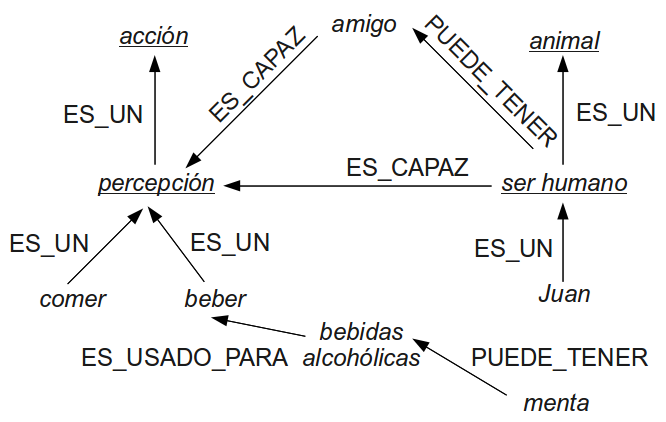
\includegraphics[width=11.019cm,height=6.969cm]{Capitulo2-img12.png}\end{minipage}
\end{center}
{\selectlanguage{spanish}\sffamily
\textstylebibuscitbase{\foreignlanguage{spanish}{Desambiguaci\'on del
sentido de las palabras utilizando la estructura de v\'inculos de
Wikipedia
}}\textstylebibuscitbase{\foreignlanguage{spanish}{(Mihalcea2007)}}}


\bigskip

{\selectlanguage{spanish}\sffamily
Utilizando \textstylebibuscitbase{los hiperv\'inculos de Wikipedia se
puede crear un corpora de sentidos etiquetado que puede ser utilizado
para construir clasificadores de sentidos
}\textstylebibuscitbase{exactos y robustos. Por medio de experimentos
de desambiguaci\'on de sentidos }\textstylebibuscitbase{de las palabras
para el corpus Wikipedia de sentidos etiquetado generado para un
subconjunto de palabras ambiguas de SENSEVAL}\footnote{El prop\'osito
de SENSEVAL es realizar ejercicios de evaluaci\'on para el an\'alisis
sem\'antico de textos de las fortalezas y debilidades de los programas
\'utiles para determinar autom\'aticamente el sentido de las palabras
en un contexto.}\textstylebibuscitbase{, se demuestra que las
anotaciones de Wikipedia son fiables}\textstylebibuscitbase{ y la
calidad del clasificador de etiquetaci\'on de sentidos construido sobre
estos datos excede en mucho la precisi\'on de una base inicial }%
%Baseline, revisar fuente
%Pendiente de completar
\textstylebibuscitbase{que selecciona el sentido de la palabra m\'as
}\textstylebibuscitbase{frecuente por default.}}


\bigskip

\subsubsection[Wikificaci\'on de Textos,
Wikify!]{\selectlanguage{spanish}\sffamily\itshape Wikificaci\'on de
Textos, Wikify!}
{\selectlanguage{spanish}\sffamily
Su prop\'osito es a\~nadir informaci\'on adicional a un texto, mediante
la obtenci\'on de sus palabras relevantes, para asociarles enlaces o
hiperv\'inculos a art\'iculos de Wikipedia (Mihalcea2007).}

{\selectlanguage{spanish}\sffamily
La Wikificaci\'on de textos se realiza en base a dos tareas:}

\liststyleLxii
\begin{enumerate}
\item {\selectlanguage{spanish}\sffamily
Extracci\'on de texto.}
\item {\selectlanguage{spanish}\sffamily
Desambiguaci\'on del sentido de las palabras.}
\end{enumerate}

\bigskip

{\selectlanguage{spanish}\sffamily
\foreignlanguage{spanish}{De los textos se extraen las palabras m\'as
relevantes, como pueden t\'erminos t\'ecnicos, entidades con nombre,
nueva terminolog\'ia y aquellos que tie}nen relaci\'on estrecha con el
texto.}

{\selectlanguage{spanish}\sffamily
La extracci\'on de textos utiliz\'o un vocabulario controlado de frases
clave de los t\'itulos de los art\'iculos de Wikipedia y de las
{\textquotedblleft}formas superficie{\textquotedblright} de los
art\'iculos de Wikipedia. Se utilizaron tres algoritmos no supervisados
para la extracci\'on de palabras clave: \textit{tf.idf},  $\chi 2$ y el
m\'etodo de Clasificaci\'on (Ranking) \textit{keyphraseness}\textit{.}}


\bigskip

{\selectlanguage{spanish}\sffamily
Posteriormente para elegir la p\'agina que se ha de asociar a las
palabras relevantes y a una p\'agina Wikipedia, se requiere de un
proceso de desambiguaci\'on, el cual se debe dar de acuerdo al contexto
en el que se encuentra cada palabra.}

{\selectlanguage{spanish}\sffamily
Agregar la imagen de la arquitectura del sistema Wikify!}


\bigskip

{\selectlanguage{spanish}\sffamily
Para la evaluaci\'on de los resultados obtenidos de los algoritmos de
extracci\'on, se creo un est\'andar de oro con un conjunto de 85
documentos y 7,286 conceptos vinculados anotados de forma manualmente,
contra el cual se compararon los t\'erminos autom\'aticamente
extra\'idos. El desempe\~no se evalu\'o en t\'erminos de precisi\'on,
memoria (recall) y medida-F (F-measure).}

{\selectlanguage{spanish}\sffamily
En cuanto a la desambiguaci\'on de palabras se utilizaron dos m\'etodos,
uno del tipo del algoritmo de Lesk, que identifica el significado m\'as
parecido de una palabra en un determinado contexto bas\'andose en una
medida de traslape contextual entre las definiciones del diccionario de
la palabra ambigua. El segundo m\'etodo es de datos dirigidos, que
incorpora caracter\'isticas locales y de inter\'es actual en un
clasificador Naive Bayes.}


\bigskip

{\selectlanguage{spanish}\sffamily
Para evaluar esta fase se realiz\'o un est\'andar de oro de un conjunto
de datos de la la misma colecci\'on de 85 p\'aginas de Wikipedia y
7,286 conceptos vinculados, con anotaciones manuales de sentidos
correspondientes a los v\'inculos.}

\clearpage\subsubsection[Identificaci\'on de temas en base a un
algoritmo de centralidad de un grafo
ensayado]{\selectlanguage{spanish}\sffamily\itshape Identificaci\'on de
temas en base a un algoritmo de centralidad de un grafo ensayado}

\bigskip

{\selectlanguage{spanish}\sffamily
Utiliza el m\'etodo no supervisado Wikify! (MihalceaCsomai2007) para
encontrar temas o categor\'ias relevantes en un documento utilizando un
algoritmo de centralidad en el grafo ensayado construido de Wikipedia.}

{\selectlanguage{spanish}\sffamily
Se toma como premisa que el conocimiento enciclop\'edico externo puede
utilizarse para identificar temas relevantes de un documento
(Mihalcea2009). Se \ realizan dos tareas:}


\bigskip

\liststyleLxiii
\begin{enumerate}
\item {\selectlanguage{spanish}\sffamily
Se construye un grafo que incluye toda la informaci\'on de la Wikipedia
en ingl\'es, los nodos equivalen a las categor\'ias y art\'iculos, los
arcos representan las relaciones de proximidad entre art\'iculos (5.8
milliones de nodos y 65.5 millones de arcos ).}
\item {\selectlanguage{spanish}\sffamily
Por cada documento, se identifica el concepto enciclop\'edico en el
texto y se crea un v\'inculo entre el contenido del art\'iculo y el
grafo enciclop\'edico externo. Se hace entonces una clasificaci\'on
utilizando una variaci\'on del algoritmo de centralidad para grafos
ensayados PageRank\footnote{Algoritmo de an\'alisis de v\'inculos que
asigna un valor num\'erico (peso) a cada elemento de un conjunto de
documentos vinculados (hiperv\'inculos) y de este modo determinar la
relevancia relativa de cada documento del conjunto. Google tiene la
marca registrada {\textquotedbl}PageRank{\textquotedbl} aunque la
patente del algoritmo es propiedad de la Universidad de Stanford. }
\ \ que }
\end{enumerate}

\bigskip

{\selectlanguage{spanish}\sffamily
\textstylebibuscitbase{Next, we run a biased graph centrality algorithm
on }}

{\selectlanguage{spanish}\sffamily
\textstylebibuscitbase{the entire graph, so that all the nodes in the
exter- }}

{\selectlanguage{spanish}\sffamily
\textstylebibuscitbase{nal knowledge repository are ranked based on
their }}

{\selectlanguage{spanish}\sffamily
\textstylebibuscitbase{relevance to the input document. We use a
variation }}

{\selectlanguage{spanish}\sffamily
\textstylebibuscitbase{of the PageRank (Brin and Page, 1998) algorithm,
}}

{\selectlanguage{spanish}\sffamily
\textstylebibuscitbase{which accounts for both the relation between the
}}

{\selectlanguage{spanish}\sffamily
\textstylebibuscitbase{nodes in the document and the encyclopedic graph,
}}

{\selectlanguage{spanish}\sffamily
\textstylebibuscitbase{as well as the relation between the nodes in the
en- }}

{\selectlanguage{spanish}\sffamily
\textstylebibuscitbase{cyclopedic graph itself. }}

{\selectlanguage{spanish}\sffamily
2.3.1 Wikipedia como base de conocimiento}


\bigskip

{\selectlanguage{spanish}\sffamily
\textstylebibuscitbase{\foreignlanguage{spanish}{Desde el punto de vista
computacional, Wikipedia constituye una base de conocimiento. Las
}}\textstylebibuscitbase{\foreignlanguage{spanish}{bases de
conocimiento para PLN deben reunir algunas
}}\textstylebibuscitbase{\foreignlanguage{spanish}{caracter\'isticas
como: ser independientes del dominio, actualizadas
}}\textstylebibuscitbase{\foreignlanguage{spanish}{frecuentemente,
multiling\"ues, las cu\'ales posee la
}}\textstylebibuscitbase{\foreignlanguage{spanish}{Wikipedia, lo que la
convierte en un recurso importante en aplicaciones de PLN.}}}


\bigskip

{\selectlanguage{spanish}\sffamily
\textstylebibuscitbase{\foreignlanguage{spanish}{Como ya se ha
mencionado, el sistema de categor\'ias de Wikipedia es considerado una
taxonom\'ia al igual que la de WordNet, esto ha permitido que ambas
sean explotadas para calcular medidas sobre proximidad sem\'antica y
similitud sem\'antica, con el prop\'osito de permitir a las
computadoras razonar sobre un texto escrito [10] y derivar
conocimiento.}}}


\bigskip

{\selectlanguage{spanish}\sffamily
Extracci\'on de conocimiento l\'exico-sem\'antico}


\bigskip

{\selectlanguage{spanish}\sffamily
\textstylebibuscitbase{\foreignlanguage{spanish}{As\'i como Wikipedia,
tambi\'en
Wiktionary}}\footnote{http://www.wiktionary.org/}\textstylebibuscitbase{\foreignlanguage{spanish}{
es considerada una base de conocimiento, ambas se han construido por
medio de la colaboraci\'on de usuarios. Se les denomina Bases de
Conocimiento Colaborativo, a diferencia de lo que se conoce como Bases
de Conocimiento Ling\"u\'istico (WordNet es un ejemplo de este
tipo).}}}


\bigskip

{\selectlanguage{spanish}\sffamily
\textstylebibuscitbase{\foreignlanguage{spanish}{Wiktionary es la parte
l\'exica de Wikipedia, y las entradas a\~nadidas incluyen informaci\'on
l\'exico-sem\'antico como parte-del-discurso, sentido de las palabras,
glosas, etimolog\'ia, pronunciaci\'on, ejemplos, traducci\'on,
colocaci\'on, t\'erminos derivados. Tambi\'en se incluye sin\'onimos,
ant\'onimos, hiper\'onimos e hip\'onimos. A diferencia de las bases de
conocimiento ling\"u\'istico incluye informaci\'on como abreviaciones,
acr\'onimos, pronunciaci\'on correcta, contracciones, proverbios,
onomatopeyas, jerga coloquial, entre otras.}}}


\bigskip

\subsubsection[Relaciones Sem\'anticas en
Wikipedia]{\selectlanguage{spanish}\sffamily\itshape Relaciones
Sem\'anticas en Wikipedia}

\bigskip

{\selectlanguage{spanish}\sffamily
\textstylebibuscitbase{\foreignlanguage{spanish}{Como se ha explicado,
Wikipedia se compone de art\'iculos, vinculados a otros art\'iculos y
organizados mayormente por medio de Categor\'ias. De estas estructuras
se ha observado que, adem\'as de las relaciones que se establecen solo
por estas estructuras, se pueden encontrar relaciones sem\'anticas.}}}


\bigskip

{\selectlanguage{spanish}\sffamily
\textstylebibuscitbase{\foreignlanguage{spanish}{En algunos trabajos se
buscan relaciones sem\'anticas fuertes
}}\textstylebibuscitbase{\foreignlanguage{spanish}{(Chernov et al.,
2006)}}\textstylebibuscitbase{\foreignlanguage{spanish}{, en la que por
medio de un esquema de base de datos se establecen relaciones que se
consideran importantes entre las categor\'ias.}}}


\bigskip

\subsubsection[Proximidad
sem\'antica]{\selectlanguage{spanish}\sffamily\itshape Proximidad
sem\'antica}
\hypertarget{RefHeading10786782078703}{}
\bigskip

{\selectlanguage{spanish}\sffamily
\textstylebibuscitbase{\foreignlanguage{spanish}{Este modelo est\'a
relacionado con el conocimiento sem\'antico. Se requiere para
desambiguar oraciones completas, porque sus diversas estructuras
sint\'acticas son perfectamente posibles, o para enlazar frases
circunstanciales que al no estar directamente enlazados con el sentido
del lexema rector requieren un m\'etodo conectado con la sem\'antica de
contexto. }}}


\bigskip

{\selectlanguage{spanish}\sffamily
\textstylebibuscitbase{\foreignlanguage{spanish}{El c\'alculo de
proximidad sem\'antica determina que tan relacionados est\'an dos
}}\textstylebibuscitbase{\foreignlanguage{spanish}{conceptos en una
taxonom\'ia por medio de las relaciones que existan entre ellos.
}}\textstylebibuscitbase{\foreignlanguage{spanish}{Es una tarea
\'util}}\textstylebibuscitbase{\foreignlanguage{spanish}{ en
aplicaciones del PLN como recuperaci\'on de informaci\'on, correcci\'on
ortogr\'afica y desambiguaci\'on del sentido de las
}}\textstylebibuscitbase{\foreignlanguage{spanish}{palabras.}}}


\bigskip

{\selectlanguage{spanish}\sffamily
\textstylebibuscitbase{\foreignlanguage{spanish}{Para realizar estos
c\'alculos se analizan las relaciones entre palabras, las m\'as comunes
son:}}}


\bigskip

\liststyleWWviiiNumxvi
\begin{itemize}
\item {\selectlanguage{spanish}\sffamily
\textstylebibuscitbase{\foreignlanguage{spanish}{antonimia}}}
\item {\selectlanguage{spanish}\sffamily
\textstylebibuscitbase{\foreignlanguage{spanish}{hiponimia/hiperonimia}}}
\item {\selectlanguage{spanish}\sffamily
\textstylebibuscitbase{\foreignlanguage{spanish}{meronimia}}}
\item {\selectlanguage{spanish}\sffamily
\textstylebibuscitbase{\foreignlanguage{spanish}{relaciones funcionales
como parte-de, hecho-de, es-un-atributo-de, etc..}}}


\bigskip

{\selectlanguage{spanish}\sffamily
\textstylebibuscitbase{\foreignlanguage{spanish}{Es usual que las
medidas de proximidad sem\'antica sean evaluadas, esto es, se compara
los resultados obtenidos con un {\textquotedblleft}est\'andar de
oro{\textquotedblright} producto del juicio humano, es decir, personas
que en base a su juicio determinan la proximidad de pares de
palabras.}}}
\end{itemize}

\bigskip

{\selectlanguage{spanish}\sffamily
Est\'andares de oro para evaluaci\'on de Proximidad Sem\'antica y
Similitud Sem\'antica}


\bigskip

{\selectlanguage{spanish}\sffamily
Uno de las m\'etodos de evaluar las medidas de proximidad sem\'antica ,
es compar\'andolas con juicios humanos, es decir, personas que realizan
un juicio sobre el grado de relaci\'on entre pares de palabras, de lo
cu\'al se obtiene un est\'andar de oro . Sobre las investigaciones de
proximidad sem\'antica y similitud sem\'antica algunos de los
est\'andares de oro utilizados son:}


\bigskip

{\selectlanguage{spanish}\sffamily
Colecci\'on WordSimilarity-353}


\bigskip

{\selectlanguage{spanish}\sffamily
Contiene dos conjuntos de pares de palabras con las anotaciones humanas
sobre similitud. Uno de los conjuntos contiene 153 pares de palabras
con su valor de similitud asignado para 13 materias. El segundo
conjunto contiene 200 pares de palabras, con la similitud resultado de
la valoraci\'on de 16 \ materias. Un tercer conjunto se conforma por
los dos conjuntos anteriores, el cual se integra por 353 palabras con
los valores de similitud.}


\bigskip

{\selectlanguage{spanish}\sffamily
\foreignlanguage{spanish}{Los conjuntos pueden descargarse
libremente}\footnote{\ http://www.cs.technion.ac.il/\~{}gabr/resources/data/wordsim353/wordsim353.html}\foreignlanguage{spanish}{
y est\'an disponibles en dos tipos }\foreignlanguage{spanish}{de
formatos:}}


\bigskip

\liststyleWWviiiNumxii
\begin{itemize}
\item {\selectlanguage{spanish}\sffamily
Valores separados por comas (Comma-separated values- CSV).}
\item {\selectlanguage{spanish}\sffamily
Delimitados por tabuladores (Tab-delimited -- TAB).}
\end{itemize}

\bigskip

{\selectlanguage{spanish}\sffamily
RG (Rubenstein \& Goodenough)}


\bigskip

{\selectlanguage{spanish}\sffamily
\foreignlanguage{spanish}{Contiene 65 pares de sustantivos, los cuales
fueron recopilados en 1965, escritos en
}\foreignlanguage{spanish}{tarjetas de papel que ten\'ian que ser
ordenadas de acuerdo a la similitud de su significado, es decir, basado
en sinonimia en vez de proximidad y
}\foreignlanguage{spanish}{calificados en una escala de 0 a 4 por 51
personas
}\textstylebibuscitbase{\foreignlanguage{spanish}{[24]}}\foreignlanguage{spanish}{.}}


\bigskip

{\selectlanguage{spanish}\sffamily
MC (Miller \& Charles)}


\bigskip

{\selectlanguage{spanish}\sffamily
Subconjunto de 30 pares de RG (Rubenstein \& Goodenough) con 38 temas de
prueba.}


\bigskip

{\selectlanguage{spanish}\sffamily
R (Resnick)}


\bigskip

{\selectlanguage{spanish}\sffamily
Replic\'o las clasificaciones del conjunto MC utilizando a 10 personas
para la calificaci\'on.}

%
%INTRODUCIR INVESTIGACIONES SOBRE PROXIMIDAD SEM\'ANTICA EN WIKIPEDIA


\subsubsection[Wikirelate!]{Wikirelate!}
\hypertarget{RefHeading335057232820}{}
\bigskip

{\selectlanguage{spanish}\sffamily
Considera el \'arbol de categor\'ias de Wikipedia como una Folksonom\'ia
resultante de la clasificaci\'on colaborativa, en la que los usuarios
pueden categorizar el contenido de las entradas enciclop\'edicas. Las
categor\'ias constituyen una red sem\'antica en la que los conceptos se
relacionan. Esta red de categor\'ias se utiliza para calcular la
proximidad sem\'antica.}


\bigskip

{\selectlanguage{spanish}\sffamily
Aplica a la Wikipedia las medidas para c\'alculo de proximidad
sem\'antica desarrolladas originalmente para WordNet:}


\bigskip

\liststyleWWviiiNumvi
\begin{enumerate}
\item {\selectlanguage{spanish}\sffamily
Medidas basadas en recorridos.}
\item {\selectlanguage{spanish}\sffamily
Medidas basadas en contenido de informaci\'on.}
\item {\selectlanguage{spanish}\sffamily
Medidas basadas en traslape de textos.}
\end{enumerate}

\bigskip

{\selectlanguage{spanish}\sffamily
El proceso de miner\'ia de este modelo consiste en tomar pares de
palabras i, j, recuperar las p\'aginas de Wikipedia a las que estas se
refieren, posteriormente se asocian al \'arbol de categor\'ias
extrayendo las categor\'ias a las que las p\'aginas recuperadas
pertenecen para finalmente calcular la proximidad sem\'antica de
acuerdo a las p\'aginas extra\'idas y las rutas encontradas sobre la
taxonom\'ia de categor\'ias.}

{\selectlanguage{spanish}\sffamily
Modelo de Vector de V\'inculos de Wikipedia (Wikipedia Link Vector Model
-- WLVM)}


\bigskip

{\selectlanguage{spanish}\sffamily
Al identificar la proximidad sem\'antica de t\'erminos y conceptos en
Wikipedia se puede extraer un tesauro como mapa de relaciones
sem\'anticas entre palabras y frases para recuperaci\'on de
informaci\'on.}


\bigskip

{\selectlanguage{spanish}\sffamily
El modelo WLVM utiliza la estructura de hiperv\'inculos de Wikipedia en
vez de utilizar contenidos textuales para el c\'alculo de medidas de
proximidad sem\'antica. El proceso de extracci\'on en este modelo
consiste en tomar pares de t\'erminos de la estructura de
hiperv\'inculos de Wikipedia. El procedimiento es extraer todos los
art\'iculos relacionados a cada t\'ermino, para lo cu\'al se realiza el
listado de todas las p\'aginas cuyos t\'itulos coincidan con el
t\'ermino y procesarlos de modo que:}


\bigskip

\liststyleLxiv
\begin{itemize}
\item {\selectlanguage{spanish}\sffamily
Los art\'iculos se usen directamente.}
\item {\selectlanguage{spanish}\sffamily
Se siguen los v\'inculos de redirecci\'on, de modo que se utilizan los
art\'iculos correspondientes.}
\item {\selectlanguage{spanish}\sffamily
Se procesan las p\'aginas de desambiguaci\'on%
%Revisar fuente
, de modo que cada art\'iculo al que vinculan sea utilizado.}
\end{itemize}

\bigskip

{\selectlanguage{spanish}\sffamily
Lo siguiente es obtener la similitud entre los t\'erminos juzgando la
similitud de las p\'aginas obtenidas previamente. La similitud
sem\'antica entre dos art\'iculos de Wikipedia se define por el
\'angulo formado por los vectores de los v\'inculos encontrados entre
ellos. Este enfoque es similar al modelo de espacio de vectores%
%Revisar traducci\'on
 utilizado en recuperaci\'on de informaci\'on. Particularmente en el
modelo WLVM los vectores no se construyen por medidas de probabilidad
como TF-IDF sino usando el peso de los valores de los v\'inculos que se
obtiene por la probabilidad de ocurrencia de cada v\'inculo definida
por el n\'umero total de v\'inculos al art\'iculo sobre el n\'umero
total de art\'iculos.}


\bigskip

{\selectlanguage{spanish}\sffamily
\foreignlanguage{spanish}{La proximidad sem\'antica m\'as alta para los
art\'iculos est\'a dada por el \'angulo m\'as peque\~no entre vectores,
que va desde los 0{\textdegree} si los art\'iculos contienen una
}\foreignlanguage{spanish}{lista id\'entica de v\'inculos, a
90{\textdegree} si no existe traslape entre ellos. As\'i se da la
desambiguaci\'on de art\'iculos, de modo que solo los dos art\'iculos
que est\'an m\'as relacionados son los utilizados como medida de
similitud. El m\'etodo para evaluar estas medidas
}\foreignlanguage{spanish}{fue compar\'andolas
con}\foreignlanguage{spanish}{
WordSimilarity-353}\footnote{http://www.cs.technion.ac.il/\~{}gabr/resources/data/wordsim353/wordsim353.html}\foreignlanguage{spanish}{.}}


\bigskip

{\selectlanguage{spanish}\sffamily
\foreignlanguage{spanish}{Otra medida de proximidad sem\'antica evaluada
con este modelo }\foreignlanguage{spanish}{se obtuvo
al}\foreignlanguage{spanish}{ sumar }\foreignlanguage{spanish}{los
pesos de los}\foreignlanguage{spanish}{ v\'inculos compartidos con
mejores resultados sobre proximidad sem\'antica entre t\'erminos,
mientras que el m\'etodo WLVM aplicado tal cual, result\'o tener
mejores resultados de proximidad sem\'antica entre
}\foreignlanguage{spanish}{art\'iculos
}\textstylebibuscitbase{\foreignlanguage{spanish}{(Milne2007)}}\foreignlanguage{spanish}{.}}


\bigskip

{\selectlanguage{spanish}\sffamily
Para desarrollar este modelo se utiliz\'o la herramienta Wikipedia Miner
desarrollada en espec\'ifico para la exploraci\'on de la estructura de
hiperv\'inculos de Wikipedia. }

{\selectlanguage{spanish}\sffamily
Modelo de Medidas basadas en V\'inculos de Wikipedia (Wikipedia
Link-based Measure - WLM)}


\bigskip

{\selectlanguage{spanish}\sffamily
\foreignlanguage{spanish}{C\'alculo de medidas de proximidad entre
art\'iculos
}\textstylebibuscitbase{\foreignlanguage{spanish}{(Milne\_2008)}}\foreignlanguage{spanish}{:}}


\bigskip

\liststyleLxv
\begin{enumerate}
\item {\selectlanguage{spanish}\sffamily
basada en los v\'inculos que se extienden hacia afuera de los
art\'iculos, esto se hace calculando el \'angulo entre vectores de los
v\'inculos encontrados en dos art\'iculos, esto es similar a los que se
hace con los vectores TF-IDF utilizados en los modelos de RI. La
diferencia radica en que se utiliza el valor del c\'omputo de pesos de
v\'inculos, en vez del c\'omputo de los pesos de la ocurrencia de
t\'erminos. Esta probabilidad se define por el n\'umero total de
v\'inculos al art\'iculo objetivo sobre el total del n\'umero de
art\'iculos. Esto es, si s y t son el art\'iculo fuente y el art\'iculo
objetivo respectivamente, entonces el peso w del v\'inculo s
$\rightarrow $ t est\'a definido por:}
\end{enumerate}

\bigskip

{\centering  $w(s\rightarrow t)=\log (\frac{W}{T})\mathit{si}s\in
T,0\mathit{de}\mathit{otro}\mathit{modo}$\par}


\bigskip

{\selectlanguage{spanish}\sffamily
donde T es el conjunto de todos los art\'iculos que se vinculan a t y W
es el conjunto de todos los art\'iculos de Wikipedia. Los pesos de los
v\'inculos se utilizan para generar los vectores correspondientes, la
similitud de los art\'iculos es el \'angulo entre vectores (similitud
por cosenos). El rango va de los 0{\textdegree} si el art\'iculo
contiene una lista id\'entica de v\'inculos a 90{\textdegree} si no
existe traslape entre ellos.}


\bigskip

\liststyleLxv
\setcounter{saveenum}{\value{enumi}}
\begin{enumerate}
\setcounter{enumi}{\value{saveenum}}
\item {\selectlanguage{spanish}\sffamily
La segunda m\'etrica que utiliza el modelo est\'a basada en las
ocurrencias de un t\'ermino en p\'aginas web, tal como ser\'ia el
resultado de b\'usquedas en el motor de Google que obtiene p\'aginas
donde ocurren los t\'erminos, pero en vez de utilizar los resultados de
b\'usqueda de Google, esta m\'etrica se basa en la estructura de
v\'inculos de Wikipedia.}

{\centering 
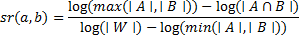
\includegraphics[width=7.909cm,height=0.979cm]{Capitulo2-img13.png}
\par}
\end{enumerate}

\bigskip

{\selectlanguage{spanish}\sffamily
donde a y b son dos art\'iculos, A y B son conjuntos de todos los
art\'iculos vinculados a a y b respectivamente y W \ es la totalidad de
Wikipedia.}


\bigskip

\subsubsection[An\'alisis Sem\'antico Expl\'icito (Explicit Semantic
Analysis {}-- ESA)]{An\'alisis Sem\'antico Expl\'icito (Explicit
Semantic Analysis -- ESA)}
\hypertarget{RefHeading10788782078703}{}
\bigskip

{\selectlanguage{spanish}\sffamily
Propone un m\'etodo que representa el significado de cualquier texto en
t\'erminos de conceptos de Wikipedia. A diferencia de los m\'etodos de
proximidad sem\'antica basados en WordNet que se limitan a proximidad
de palabras, este m\'etodo calcula la proximidad de textos
arbitrarios.}


\bigskip

{\selectlanguage{spanish}\sffamily
Utiliza t\'ecnicas de m\'aquinas de aprendizaje (machine learning) para
representar el significado de los t\'erminos(textos) como vectores de
los conceptos de Wikipedia, llamados vectores de interpretaci\'on, los
cuales tienen asignados pesos utilizando TF-IDF.}


\bigskip

{\selectlanguage{spanish}\sffamily
Se eval\'uan los resultados calculando autom\'aticamente el grado de
proximidad sem\'antica entre fragmentos de textos de lenguaje natural,
comparando los vectores usando la m\'etrica de cosenos.}


\bigskip

{\selectlanguage{spanish}\sffamily
En correlaci\'on con m\'etodos de proximidad sem\'antica humanos se
observan mejoras de r =0.56 a 0.75 para palabras, y de r =0.60 a 0.72
para textos.}


\bigskip

\subsection[Wikipedia como red sem\'antica]{Wikipedia como red
sem\'antica}
\hypertarget{RefHeading10790782078703}{}
\bigskip

{\selectlanguage{spanish}\sffamily
\foreignlanguage{spanish}{Para calcular la proximidad sem\'antica entre
palabras, se puede utilizar el sistema de categorizaci\'on de Wikipedia
como una red sem\'antica
}\textstylebibuscitbase{\foreignlanguage{spanish}{(Ponzetto\&Strube)}}\foreignlanguage{spanish}{.}}

{\selectlanguage{spanish}\sffamily
Wikipedia como \textit{corpus} de entrenamiento}


\bigskip

{\selectlanguage{spanish}\sffamily
Wikipedia ha sido utilizada como \textit{corpus} de entrenamiento para
categorizaci\'on de temas de recursos de aprendizaje
\textstylebibuscitbase{(Meyer2007)}, se utiliza el m\'etodo de
comparaci\'on de proximidad de vecinos, (k-Nearest-Neighbors)%
%Se elimino parrafo en ingles que falta incluir
 para categorizar los recursos de aprendizaje con art\'iculos de
Wikipedia.}


\bigskip

{\selectlanguage{spanish}\sffamily
Los art\'iculos se transforman a un vector de palabras, los recursos son
mapeados a vectores de palabras para compararlos. Los vectores
similares se considera que cubren temas similares. La categorizaci\'on
de los recursos de aprendizaje, en este caso, de objetos de
aprendizaje, se hace tomando el sistema de categor\'ias de Wikipedia
como base.}


\bigskip

{\selectlanguage{spanish}\sffamily
El procesamiento de todas las categor\'ias de Wikipedia, como muchos de
los procesos que explotan su informaci\'on, consume muchos recursos de
c\'omputo, como lo son la capacidad de memoria y la complejidad de
calculo, lo que se convierte en factores limitantes. }

\subsubsection[Wikipedia como corpus XML ]{Wikipedia como corpus XML
\footnotemark{}}
\hypertarget{RefHeading10792782078703}{}\footnotetext{http://www-connex.lip6.fr/\~{}denoyer/wikipediaXML/}

\bigskip

{\selectlanguage{spanish}\sffamily
Wikipedia tambi\'en tiene una estructura de archivos XML. Se tiene
noci\'on de la utilizaci\'on de los archivos XML de la Wikipedia como
corpus, integrado por documentos XML de ocho colecciones en idiomas
diferentes: ingl\'es, franc\'es, alem\'an, espa\~nol, chino, \'arabe y
japon\'es. }

{\selectlanguage{spanish}\sffamily
Los textos est\'an codificados en UTF-8 resultado de los textos
originales de Wikipedia, del corpus se han eliminado textos de tipo
plantillas y de comentarios
\textstylebibuscitbase{(Denoyer2006)}\textstylebibuscitbase{. Este
recurso se ha empleado para tareas de recuperaci\'on de informaci\'on,
como son recuperaci\'on ad-hoc, categorizaci\'on, clustering y tareas
de mapeo de estructuras.}}


\bigskip

\subsubsection[Crear un corpus de texto plano de
Wikipedia]{\textstylebibuscitbase{Crear un
}\textstylebibuscitbase{corpus}\textstylebibuscitbase{ de texto plano
de Wikipedia}}
\hypertarget{RefHeading10794782078703}{}
\bigskip

{\selectlanguage{spanish}\sffamily
\textstylebibuscitbase{Las colecciones de texto de Wikipedia pueden
convertirse en corpus}\footnote{\foreignlanguage{english}{Extracting
Text from Wikipedia,
}\url{http://evanjones.ca/software/wikipedia2text.html}\foreignlanguage{english}{.}}\footnote{\foreignlanguage{english}{G}\foreignlanguage{english}{enerating
a Plain Text Corpus from Wikipedia,
}\url{http://blog.afterthedeadline.com/2009/12/04/generating-a-plain-text-corpus-from-wikipedia/}\foreignlanguage{english}{.}}\textstylebibuscitbase{,
como }\textstylebibuscitbase{en el caso de }\textstylebibuscitbase{los
art\'iculos Wikipedia, archivos con formato y etiquetado
MediaWiki}\footnote{http://en.wikipedia.org/wiki/MediaWiki}\textstylebibuscitbase{
y que pueden obtenerse por idioma, descargando el respaldo de la
}\textstylebibuscitbase{base de datos (dump
databases)}\footnote{http://download.wikimedia.org/backup-index.html}\textstylebibuscitbase{
correspondiente.}}


\bigskip

{\selectlanguage{spanish}\sffamily
\textstylebibuscitbase{De manera general el procedimiento consiste en
descargar el respaldo conveniente, los cuales son documentos de
tama\~no considerable y por estas
}\textstylebibuscitbase{caracter\'isticas est\'an en formato
comprimido. Los respaldos se descomprimen y }\textstylebibuscitbase{el
contenido debe ser analizados sint\'acticamente
(}\textstylebibuscitbase{\textit{parser)}}\textstylebibuscitbase{ para
cambiar la sintaxis }\textstylebibuscitbase{propia
}\textstylebibuscitbase{de marcas de los art\'iculos Wiki y obtener
otro tipo de archivo (i.e. XML o texto plano).}}


\bigskip

{\selectlanguage{spanish}\sffamily
\textstylebibuscitbase{Ejemplos del procedimiento para obtener un corpus
de este tipo pueden }\textstylebibuscitbase{encontrarse en internet, el
respaldo de la base de datos (Dump) del idioma ingl\'es es el m\'as
explotado, pero pueden encontrarse inclusive en idioma
}\textstylebibuscitbase{noruego}\footnote{\url{https://www.hf.ntnu.no/hf/isk/Ansatte/petter.haugereid/cl/wiki-corpus.html}\foreignlanguage{english}{.}}\textstylebibuscitbase{.}}


\bigskip

{\selectlanguage{spanish}\sffamily
\textstylebibuscitbase{La tarea m\'as complicada de este proceso es la
del an\'alisis sint\'actico, sin }\textstylebibuscitbase{embargo,
existen varios proyectos de
parsers}\footnote{http://www.mediawiki.org/wiki/Alternative\_parsers}\textstylebibuscitbase{
alternativos al de MediaWiki adem\'as del propio.}}


\bigskip

\subsubsection[Wikicorpus (Reese2010)]{\textstylebibuscitbase{Wikicorpus
}\textstylebibuscitbase{(Reese2010)}}
\hypertarget{RefHeading10796782078703}{}
\bigskip

{\selectlanguage{spanish}\sffamily
\textstylebibuscitbase{Se trata de otro proyecto de corpus producto de
porciones de Wikipedia y enriquecido con informaci\'on ling\"u\'istica,
triling\"ue (catal\'an, espa\~nol, ingl\'es) con alrededor de 750
millones de palabras. Es un corpora anotado, con lemas y categor\'ias
gramaticales (part-of-speech) usando la libreria de c\'odigo abierto
FreeLing}\footnote{FreeLing: An Open Source Suite of Language
Analyzers, http://nlp.lsi.upc.edu/freeling/}\textstylebibuscitbase{ que
es una librer\'ia orientada al desarrollo que proporciona servicios de
an\'alisis del lenguaje. Tambi\'en est\'a anotado con sentidos por
medio del Estado del Arte del algoritmo de Desambiguaci\'on de Sentidos
de las Palabras UKB que asigna anotaciones de WordNet. El algoritmo
UKB}\footnote{\foreignlanguage{spanish}{\textrm{UKB: Graph Based Word
Sense Disambiguation and Similarity,
}}http://ixa2.si.ehu.es/ukb/}\textstylebibuscitbase{\foreignlanguage{spanish}{
se basa en una red de relaciones sem\'anticas para eliminar la
ambig\"uedad de los sentidos m\'as
}}\textstylebibuscitbase{\foreignlanguage{spanish}{probables de las
palabras en un texto utilizando el algoritmo de Clasificaci\'on de
P\'aginas (PageRank).}}}


\bigskip

{\selectlanguage{spanish}\sffamily
\textstylebibuscitbase{El proyecto Wikicorpus tiene dos prop\'ositos
principales:}}


\bigskip

\liststyleLxvi
\begin{enumerate}
\item {\selectlanguage{spanish}\sffamily
\textstylebibuscitbase{Poner a disposici\'on un corpus enriquecido con
informaci\'on ling\"u\'istica,}}
\item {\selectlanguage{spanish}\sffamily
\textstylebibuscitbase{Explorar la inducci\'on de recursos l\'exico
sem\'anticos multiling\"ues.}}
\end{enumerate}

\bigskip

{\selectlanguage{spanish}\sffamily
\textstylebibuscitbase{Como parte del proceso de obtenci\'on del corpus
se desarrollaron dos productos }\textstylebibuscitbase{disponibles para
PLN: un parser de p\'aginas de Wikipedia desarrollado en Java
}\textstylebibuscitbase{y la integraci\'on de un algoritmo de
desambiguaci\'on sem\'antica al FreeLing.}}


\bigskip

{\selectlanguage{spanish}\sffamily
\textstylebibuscitbase{El corpus se obtuvo mediante tres subprocesos:}}


\bigskip

\liststyleLxvii
\begin{enumerate}
\item {\selectlanguage{spanish}\sffamily
\textstylebibuscitbase{Filtrado, mediante el cual se excluyeron
p\'aginas sin categor\'ia, como son las p\'aginas de redirecci\'on.}}
\item {\selectlanguage{spanish}\sffamily
\textstylebibuscitbase{Extracci\'on de texto, utilizando el parser
JavaCC que se desarroll\'o espec\'ificamente para la obtenci\'on del
corpus.}}
\item {\selectlanguage{spanish}\sffamily
\textstylebibuscitbase{Procesamiento ling\"u\'istico de los textos
utilizando FreeLing para lo cual fueron tokenizados, lematizados y
etiquetados con }\textstylebibuscitbase{partes del
discurso}\textstylebibuscitbase{. }\textstylebibuscitbase{Adem\'as se
integr\'o el algoritmo para desambiguaci\'on sem\'antica basado en
grafos UKB.}}
\end{enumerate}

\bigskip

\subsubsection[Wikitology: Wikipedia como una ontolog\'ia.]{Wikitology:
Wikipedia como una ontolog\'ia.}
\hypertarget{RefHeading10798782078703}{}
\bigskip

{\selectlanguage{spanish}\sffamily
\textstylebibuscitbase{\foreignlanguage{spanish}{El proyecto Wikitology
}}\textstylebibuscitbase{\foreignlanguage{spanish}{(Syed2008)}}\textstylebibuscitbase{\foreignlanguage{spanish}{
propone un sistema para identificar temas y conceptos asociados a un
conjunto de documentos, esto es, predecir conceptos comunes a ese
conjunto utilizando la Wikipedia (versi\'on en ingl\'es) como una
ontolog\'ia, en la que sus art\'iculos y categor\'ias representan
conceptos.}}}


\bigskip

{\selectlanguage{spanish}\sffamily
\textstylebibuscitbase{\foreignlanguage{spanish}{Explota la
informaci\'on sem\'antica contenida en sus p\'aginas:}}}


\bigskip

\liststyleWWviiiNumviii
\begin{enumerate}
\item {\selectlanguage{spanish}\sffamily
\textstylebibuscitbase{\foreignlanguage{spanish}{v\'inculos desde y
hacia otros art\'iculos de Wikipedia,}}}
\item {\selectlanguage{spanish}\sffamily
\textstylebibuscitbase{\foreignlanguage{spanish}{v\'inculos a p\'aginas
de desambiguaci\'on,}}}
\item {\selectlanguage{spanish}\sffamily
\textstylebibuscitbase{\foreignlanguage{spanish}{v\'inculos de
redireccionamiento,}}}
\item {\selectlanguage{spanish}\sffamily
\textstylebibuscitbase{\foreignlanguage{spanish}{v\'inculos desde y
hac\'ia p\'aginas web externas,}}}
\item {\selectlanguage{spanish}\sffamily
\textstylebibuscitbase{\foreignlanguage{spanish}{valores calculados
PageRank calculado por motores de b\'usqueda como Google,}}}
\item {\selectlanguage{spanish}\sffamily
\textstylebibuscitbase{\foreignlanguage{spanish}{historial de p\'aginas
que indican cuando y qu\'e tan frecuente han sido editadas.}}}
\end{enumerate}
{\selectlanguage{spanish}\sffamily
\textstylebibuscitbase{\foreignlanguage{spanish}{Tambi\'en es una
fortaleza el que sus p\'aginas est\'an ligadas a ontolog\'ias formales
como DBPedia y Semantic MediaWiki, as\'i como en el sistema comercial
Freebase.}}}


\bigskip

{\selectlanguage{spanish}\sffamily
\textstylebibuscitbase{\foreignlanguage{spanish}{Este sistema utiliza
los art\'iculos de Wikipedia y los grafos de categor\'ias y de
}}\textstylebibuscitbase{\foreignlanguage{spanish}{v\'inculos a los
art\'iculos para la predicci\'on de conceptos. El grafo de categor\'ias
se utiliza para la predicci\'on de conceptos generalizados y el grafo
de v\'inculos a los art\'iculos para predicci\'on de conceptos
espec\'ificos que no se encuentran en la jerarqu\'ia de categor\'ia.}}}


\bigskip

\subsubsection[APIs para Wikipedia]{APIs para Wikipedia}
\hypertarget{RefHeading10800782078703}{}
\bigskip

{\selectlanguage{spanish}\sffamily
Explorar el \'arbol de categor\'ias}


\bigskip

{\selectlanguage{spanish}\sffamily
\textstylebibuscitbase{\textcolor{black}{La herramienta
Extension:CategoryTree}}\footnote{http://www.mediawiki.org/wiki/Extension:CategoryTree}\textstylebibuscitbase{\textcolor{black}{
integrada al software de MediaWiki,
}}\textstylebibuscitbase{\textcolor{black}{permite explorar
din\'amicamente el \'arbol de categor\'ias, utiliza AJAX para cargar
las porciones del \'arbol que se est\'an explorando.}}}


\bigskip

\subsubsection[Calcular la proximidad de palabras]{Calcular la
proximidad de palabras}
\hypertarget{RefHeading10802782078703}{}
\bigskip

{\selectlanguage{spanish}\sffamily
Para calcular proximidad sem\'antica se transforman recursos l\'exicos
en una red o grafo y se calcula la proximidad utilizando rutas o
caminos o la longitud resultante del n\'umero de nodos entre los
t\'erminos de una jerarqu\'ia.}


\bigskip

{\selectlanguage{spanish}\sffamily
Esta API calcula la proximidad sem\'antica de la siguiente manera:}


\bigskip

\liststyleWWviiiNumxviii
\begin{enumerate}
\item {\selectlanguage{spanish}\sffamily
Se parte de un par de palabras como entrada,}
\item {\selectlanguage{spanish}\sffamily
Se recuperan los art\'iculos a los que hacen referencia (utilizando
estrategias de desambiguaci\'on basadas en la estructura de v\'inculos
de los art\'iculos)}
\item {\selectlanguage{spanish}\sffamily
Se calculan las rutas o caminos en el grafo de categorizaci\'on entre
las categor\'ias a las que est\'an asignados los art\'iculos,}
\item {\selectlanguage{spanish}\sffamily
Se entregan los resultados de las rutas o caminos encontrados,}
\item {\selectlanguage{spanish}\sffamily
Se califica de acuerdo a determinadas medidas definidas.}
\end{enumerate}

\bigskip

{\selectlanguage{spanish}\sffamily
\foreignlanguage{spanish}{La implementaci\'on toma como base te\'orica
c\'alculo de longitud de caminos o rutas
}\textstylebibuscitbase{\foreignlanguage{spanish}{(Syed2008)}}\foreignlanguage{spanish}{,
informaci\'on de contenidos (information-content)
}\textstylebibuscitbase{\foreignlanguage{spanish}{(Zesch2008)}}\textstylebibuscitbase{\foreignlanguage{spanish}{
}}\foreignlanguage{spanish}{y medidas de superposici\'on de texto
(text-overlap)
}\textstylebibuscitbase{\foreignlanguage{spanish}{(Milne\_2008)}}\foreignlanguage{spanish}{.}}


\bigskip

{\selectlanguage{spanish}\sffamily
Esta API implementa las clases para realizar consultas a la Wikipedia
para recuperar entradas de esta enciclopedia as\'i como determinar el
resultado de pares de palabras.}


\bigskip

\subsubsection[Sistema para indexar textos Wiki]{Sistema para indexar
textos Wiki}
\hypertarget{RefHeading10804782078703}{}
\bigskip

{\selectlanguage{spanish}\sffamily
El concepto de Wiki se refiere a un sitio web colaborativo el cual
permite la edici\'on p\'aginas web ligadas utilizando un lenguaje
simplificado de marcas o un editor de tipo \textbf{WYSIWYG}
(\textbf{\textit{W}}\textit{hat }\textbf{\textit{Y}}\textit{ou
}\textbf{\textit{S}}\textit{ee }\textbf{\textit{I}}\textit{s
}\textbf{\textit{W}}\textit{hat }\textbf{\textit{Y}}\textit{ou
}\textbf{\textit{G}}\textit{et). }Es err\'oneo referirse a la Wikipedia
como Wiki, ya que Wikipedia es un proyecto de textos o p\'aginas Wiki.
Los datos contenidos en Wikipedia est\'an divididos en textos y
v\'inculos, los cuales pueden ser[7]: }


\bigskip

\liststyleLxviii
\begin{itemize}
\item {\selectlanguage{spanish}\sffamily
internos, que son v\'inculos que ligan p\'aginas dentro de un mismo
sitio;}
\end{itemize}
\liststyleLxix
\begin{itemize}
\item {\selectlanguage{spanish}\sffamily
externos, que son v\'inculos hacia sitios externos;}
\item {\selectlanguage{spanish}\sffamily
inter wikis, especif\'ican el art\'iculo que describe un t\'ermino de la
enciclopedia pero en otro lenguaje;}
\item {\selectlanguage{spanish}\sffamily
categor\'ias, clasifican los art\'iculos tem\'aticamente.}
\end{itemize}

\bigskip

{\selectlanguage{spanish}\sffamily
Esta organizaci\'on permite distinguir tres tipos de algoritmos de
b\'usqueda:}

{\selectlanguage{spanish}\sffamily
Convertir textos Wiki en textos de Lenguaje Natural mediante el uso de
expresiones regulares realizando dos tareas: eliminaci\'on y
transformaci\'on del texto:}


\bigskip

{\selectlanguage{spanish}\sffamily
Paso 1, eliminaci\'on de etiquetas}

{\selectlanguage{spanish}\sffamily
Paso 2, transformaci\'on de etiquetas Wiki}


\bigskip

{\selectlanguage{spanish}\sffamily
\textstylebibuscitbase{\textcolor{black}{Con las Wikipedias rusa y en
ing\'es se implement\'o un sistema para indexar
}}\textstylebibuscitbase{\textcolor{black}{textos Wiki
}}\textstylebibuscitbase{\textcolor{black}{(Krizhanovsky2009)}}\textstylebibuscitbase{\textcolor{black}{
conocida como WikIDF. Para indexar la lista de lemas y la frecuencia de
su ocurrencia se utiliz\'o el sistema GATE, tambi\'en se
}}\textstylebibuscitbase{\textcolor{black}{utiliz\'o el analizador
morfol\'ogico Lemmatizer, y el m\'odulo RussianPOStagger. Al utilizar
WikIDF, se dise\~naron los \'indices DB para ambas Wikipedias.}}}


\bigskip

\subsubsection[Herramienta de miner\'ia de Wikipedia (Wikipedia Miner
Toolkit)]{\textstylebibuscitbase{\textcolor{black}{Herramienta de
miner\'ia de Wikipedia (Wikipedia Miner Toolkit)}}}
\hypertarget{RefHeading10806782078703}{}
\bigskip

{\selectlanguage{spanish}\sffamily
\textstylebibuscitbase{\textcolor{black}{Herramienta de c\'odigo
abierto}}\footnote{http://wikipedia-miner.sourceforge.net/}\textstylebibuscitbase{\textcolor{black}{
y de acceso orientado a objetos que permite consultar y desplegar
informaci\'on de la estructura y contenido de Wikipedia. Con esta
herramienta es posible comparar sem\'anticamente t\'erminos y conceptos
y detectar temas cuando son mencionados en documentos.}}}

{\selectlanguage{spanish}\sffamily
\textstylebibuscitbase{\textcolor{black}{Por medio del procesamiento de
los respaldos (dumps) de la Wikipedia se pueden extraer sumarios del
gr\'afico de hiperv\'inculos y la jerarqu\'ia de categor\'ias.}}}

{\selectlanguage{spanish}\sffamily
\textstylebibuscitbase{\textcolor{black}{La herramienta cuenta con
scripts en PERL para la extracci\'on de sumarios, se
}}\textstylebibuscitbase{\textcolor{black}{puede comunicar con la base
de datos MySQL para indexar de manera persistente la informaci\'on que
se extrae, tambi\'en incluye una API desarrollada en Java que
simplifica los datos para su acceso}}%
%\ (which abstracts away from the data to provide simplified access ).
\textstylebibuscitbase{\textcolor{black}{.}}}


\bigskip

{\selectlanguage{spanish}\sffamily
\textstylebibuscitbase{\foreignlanguage{spanish}{\textcolor{black}{Permite
el c\'alculo de proximidad sem\'antica utilizando la estructura de
hiperv\'inculos de Wikipedia (Wikipedia Link-based Measure - WLM) , con
la que se obtiene resultados m\'as precisos y menos costosos que ESA,
lo cu\'al atribuye a que la estructura de hiperv\'inculos es la
conexi\'on definida manualmente de dos conceptos desambiguados
manualmente [10], es decir, el m\'etodo est\'a m\'as cercano a la
sem\'antica definida manualmente en Wikipedia.}}}}


\bigskip

\subsubsection[Librer\'ia Wikipedia basada en Java (JWPL {}-
Java{}-based Wikipedia Library) y Librer\'ia Wiktionary basada en Java
(JWKLT {}-- Java{}-based Wiktionary Library)]{Librer\'ia Wikipedia
basada en Java (JWPL {}- \textcolor{black}{Java-based Wikipedia
Library) y Librer\'ia Wiktionary basada en Java (JWKLT -- Java-based
Wiktionary Library)}}
\hypertarget{RefHeading10808782078703}{}
\bigskip

{\selectlanguage{spanish}\sffamily
\textcolor{black}{Con respaldos (dumps) de Wikipedia
}\textstylebibuscitbase{\textcolor{black}{(Zesch2008)}}\textcolor{black}{
se importa a una base de datos, para explotar el indexado
}\textcolor{black}{de}\textcolor{black}{ la base de datos que garantiza
casi tiempo }\textcolor{black}{constante de recuperaci\'on por cada
art\'iculo. Se utiliz\'o el framework objeto-relacional de Hibernate.
La interface de programaci\'on orientada a objetos est\'a
}\textcolor{black}{centrada en los objetos:
W}\textsc{\textcolor{black}{ikipedia, Page y
Category}}\textcolor{black}{:}}


\bigskip

\begin{center}
\tablehead{}
\begin{supertabular}{|m{2.476cm}|m{11.101cm}|}
\hline
\centering \selectlanguage{spanish}\sffamily Objeto &
\centering\arraybslash \selectlanguage{spanish}\sffamily
Operaciones\\\hline
\centering \selectlanguage{spanish}\sffamily
\textcolor{black}{W}\textsc{\textcolor{black}{ikipedia}} &
\liststyleWWviiiNumx
\begin{itemize}
\item \centering\arraybslash \selectlanguage{spanish}\sffamily
Establecer la conexi\'on con la base de datos.\item
\centering\arraybslash \selectlanguage{spanish}\sffamily Iterar sobre
los art\'iculos, categor\'ias, p\'aginas de redirecci\'on y
desambiguaci\'on.\end{itemize}
\\\hline
\centering \selectlanguage{spanish}\sffamily Page &
\liststyleWWviiiNumxvii
\begin{itemize}
\item \centering\arraybslash \selectlanguage{spanish}\sffamily
Representar art\'iculos normales, p\'aginas de redirecci\'on y
desambiguaci\'on.\item \centering\arraybslash
\selectlanguage{spanish}\sffamily Proporcionar acceso al texto de un
art\'iculo (con informaci\'on de marcas o texto plano), las
categor\'ias asignadas, los v\'inculos internos y externos del
art\'iculo, v\'inculos de redirecci\'on.\end{itemize}
\\\hline
\centering \selectlanguage{spanish}\sffamily Category &
\liststyleWWviiiNumxv
\begin{itemize}
\item \centering\arraybslash \selectlanguage{spanish}\sffamily Acceder a
los art\'iculos de una categor\'ia.\item \centering\arraybslash
\selectlanguage{spanish}\sffamily Las categor\'ias al estar conformadas
como un tesauro, este objeto proporciona los m\'etodos para recuperar
categor\'ias padre e hijas.\item \centering\arraybslash
\selectlanguage{spanish}\sffamily Objeto \textsc{CategoryGraph }que
entre otras operaciones, permite encontrar la ruta m\'as corta entre
dos categor\'ias.\end{itemize}
\\\hline
\end{supertabular}
\end{center}

\bigskip

{\selectlanguage{spanish}\sffamily
\textcolor{black}{Con respaldos (dumps) de Wiktionary en formato XML en
diferentes lenguajes se hace el parseo utilizando la librer\'ia de base
de datos Berkley DB. Para cada }\textcolor{black}{entrada del
Wiktionary, la API regresa un objeto Java
}\textsc{\textcolor{black}{Wiktionary }}\textcolor{black}{para hacer
consultas a la base de datos sobre informaci\'on sobre alguna palabra
utilizando el grafema como argumento de la consulta. Adicionalmente
puede especificarse parte-del-discurso o el lenguaje de la palabra.}}


\bigskip

{\selectlanguage{spanish}\sffamily
Estas librer\'ias han sido utilizadas en investigaciones de PLN como
son:}

\liststyleWWviiiNumiv
\begin{itemize}
\item {\selectlanguage{spanish}\sffamily
\textcolor{black}{Analizar y acceder a las estructura de grafo de
categor\'ias de Wikipedia
}\textstylebibuscitbase{\textcolor{black}{(Zesch2007)}}\textcolor{black}{.}}
\item {\selectlanguage{spanish}\sffamily
C\'alculo de proximidad sem\'antica entre palabras .}
\item {\selectlanguage{spanish}\sffamily
Recuperaci\'on de informaci\'on sem\'antica.}
\end{itemize}

\bigskip

\subsubsection[WikiLibros]{WikiLibros}
\hypertarget{RefHeading10810782078703}{}
\bigskip

{\selectlanguage{spanish}\sffamily
Este proyecto (WikiProject) tiene como objetivo que los usuarios
escriban \textit{Libros-Wikipedia} (\textit{Wikipedia-Books}), en
espa\~nol el proyecto se conoce como \textit{WikiLibros. }La idea del
proyecto es permitir a los uaurios crear libros de acuerdo a sus
especificaciones utilizando el amplio banco de contenidos libres de
Wikipedia y proporcionar las reglas para utilizar la p\'agina
Wikipedia:Books, sus subp\'aginas\footnote{Wikipedia:WikiProject
Wikipedia-Books, http://en.wikipedia.org/wiki/Wikipedia:WBOOKS} y las
herramientas (Wikipedia-Books tools) que permiten crear un WikiLibro. }

{\selectlanguage{spanish}\sffamily
Un Libro-Wikipedia es una colecci\'on de art\'iculos Wikipedia que
pueden ser salvados, presentados v\'ia electr\'onica en formato
portable PDF (portable document format) o en formato abierto ODF
(OpenDocument format) u ordenado como un libro impreso.}

{\selectlanguage{spanish}\sffamily
\foreignlanguage{spanish}{La }empresa encargada de las ediciones
impresas es PediaPress (\url{http://pediapress.com/}) que se pueden
obtener dentro del mismo sitio web de Wikipedia en la secci\'on de
imprimir/exportar. El servicio tiene un costo que varia de acuerdo al
n\'umero de p\'aginas.}


\bigskip

\subsubsection[Herramienta para generar Libros (Book Tool)]{Herramienta
para generar Libros (Book Tool)\footnotemark{}}
\hypertarget{RefHeading10812782078703}{}\footnotetext{Book tool,
http://meta.wikimedia.org/wiki/Book\_tool}
{\selectlanguage{spanish}\sffamily
Esta herramienta permite a los usuarios organizar la selecci\'on de
p\'aginas que realicen en forma de libro que puede ser:}


\bigskip

\liststyleLxx
\begin{itemize}
\item {\selectlanguage{spanish}\sffamily
editado y estructurado en cap\'itulos,}
\item {\selectlanguage{spanish}\sffamily
compartido y cargado,}
\item {\selectlanguage{spanish}\sffamily
presentado como documento ODF,}
\item {\selectlanguage{spanish}\sffamily
exportado como documento ODF,}
\item {\selectlanguage{spanish}\sffamily
ser solicitado como un libro impreso a PediaPress.}
\end{itemize}

\bigskip

{\selectlanguage{spanish}\sffamily
El n\'ucleo del proyecto es todas las p\'aginas en el espacio de nombres
\textit{Book} (i.e. P\'aginas que comienzan con \textit{Book:...), }y
cualquier categor\'ia o plantilla que este relacionada con estas
p\'aginas. }

{\selectlanguage{spanish}\sffamily
El proceso de creaci\'on para usuarios normales se desagrega en cuatro
pasos\footnote{Book tool/Help/Books,
http://meta.wikimedia.org/wiki/Book\_tool/Help/Books}:}


\bigskip

\liststyleLxxi
\begin{enumerate}
\item {\selectlanguage{spanish}\sffamily
En la p\'agina de Wikipedia, en el men\'u lateral izquierdo se puede ver
el submenu de opciones Imprimir/exportar (Print/export) como se muestra
en la Figura \ref{seq:ref0}, en el cual se encuentran las opciones para
generar un WikiLibro, por medio de la opci\'on Create a book se
habilita la herramienta \textit{Book creator}, que se permanece activa
en la parte superior de las p\'aginas de Wikipedia. }
\end{enumerate}

\bigskip

\liststyleLxxi
\setcounter{saveenum}{\value{enumi}}
\begin{enumerate}
\setcounter{enumi}{\value{saveenum}}
\item {\selectlanguage{spanish}\sffamily
Las p\'aginas pueden irse agregando al libro con la opci\'on Agregar
esta p\'agina al libro (Add this page to your book) como se muestra en
la Figura \ref{seq:ref0}:}

{\selectlanguage{spanish}\sffamily
Las categor\'ias pueden tambi\'en agregarse y cada vez que se agrega una
categor\'ia todas sus p\'aginas pertenecientes se anexan al libro, esto
se hace con la opci\'on Agregar esta categor\'ia al libro (Add this
category to your book) como se aprecia en la Figura
\ref{seq:refFigura6}.}



\begin{center}
\begin{minipage}{10.583cm}
{\centering\selectlanguage{spanish}\itshape
Figura {\refstepcounter{Figura}\theFigura\label{seq:refFigura6}}:
Agregar categor\'ias a un WikiLibro.
\par}

\includegraphics[width=10.583cm,height=2.815cm]{Capitulo2-img14.png}\end{minipage}
\end{center}
{\selectlanguage{spanish}\sffamily
Una vez que se han agregado p\'aginas o categor\'ias se puede revisar el
material seleccionado con la opci\'on Show book que se puede observar
en la Figura \ref{seq:refFigura7} y se puede agregar t\'itulo y
subt\'itulos, tambi\'en se puede reorganizar el orden de los libros.}


\bigskip
\end{enumerate}


\begin{center}
\begin{minipage}{13.231cm}
{\centering\selectlanguage{spanish}\itshape
Figura {\refstepcounter{Figura}\theFigura\label{seq:refFigura7}}:
Opci\'on Show Book para visualizar el contenido del libro.
\par}

\includegraphics[width=11.458cm,height=3.046cm]{Capitulo2-img15.png}\end{minipage}
\end{center}
\liststyleLxxi
\setcounter{saveenum}{\value{enumi}}
\begin{enumerate}
\setcounter{enumi}{\value{saveenum}}
\item[] 
\bigskip

{\selectlanguage{spanish}\sffamily
El libro ya terminado puede ser descargado en formato PDF u ODF como se
ha mencionado o bien puede ordenarse una copia impresa a PediaPress, la
Figura \ref{seq:ref0} muestra como puede seleccionarse el formato en el
cual obtener el libro.}


\bigskip

{\selectlanguage{spanish}\sffamily
La creaci\'on de un WikiLibro depende de la selecci\'on de art\'iculos y
categor\'ias de Wikipedia que seleccionen los usuarios y no puede
exceder a 500 art\'iculos en tanto que los libros impresos no pueden
exceder de 800 p\'aginas impresas. Se estructuran en base a una
plantilla con la sintaxis Wiki.}


\bigskip
\end{enumerate}
\clearpage
\bigskip

{\selectlanguage{spanish}\sffamily\bfseries
Bibliograf\'ia}
{\selectlanguage{spanish}
\textstylebibusindexbase{[Buriol2006]
}\ \ \textstylebibusindexbase{Buriol Luciana S, Castillo Carlos, Donato
Debora, Leonardi Stefano \& Millozzi Stefano.
}\textstylebibusindexbasei{Temporal Analysis of the
Wikigraph}\textstylebibusindexbase{. }\textstylebibusindexbasei{Web
Intelligence, Hong Kong}\textstylebibusindexbase{ (2006)
}\textstylebibusindexbase{: }\textstylebibusindexbase{.}}

{\selectlanguage{spanish}
\textstylebibusindexbase{[Capocci2006]
}\ \ \textstylebibusindexbase{Capocci A, Servedio V D P, Colaiori F,
Buriol L S, Donato D, Leonardi S \& Caldarelli G.
}\textstylebibusindexbasei{Preferential attachment in the growth of
social networks: the case of Wikipedia\newline
}\textstylebibusindexbase{.
}\textstylebibusindexbase{\ (}\textstylebibusindexbase{2006)
}\textstylebibusindexbase{: }\textstylebibusindexbase{.}}

{\selectlanguage{spanish}
\textstylebibusindexbase{[Milne\_2008]
}\ \ \textstylebibusindexbase{David Milne \& Ian H Witten.
}\textstylebibusindexbasei{An Effective, Low-Cost Measure of Semantic
Relatedness Obtained from Wikipedia Links}\textstylebibusindexbase{.
}\textstylebibusindexbase{\ (}\textstylebibusindexbase{2008)
}\textstylebibusindexbase{: }\textstylebibusindexbase{.}}

{\selectlanguage{spanish}
\textstylebibusindexbase{[Denoyer2006]
}\ \ \textstylebibusindexbase{Denoyer Ludovic \& Gallinari Patrick.
}\textstylebibusindexbasei{The Wikipedia XML
Corpus}\textstylebibusindexbase{.
}\textstylebibusindexbase{\ (}\textstylebibusindexbase{2006)
}\textstylebibusindexbase{: }\textstylebibusindexbase{.}}

{\selectlanguage{spanish}
\textstylebibusindexbase{[Holloway]
}\ \ \textstylebibusindexbase{Holloway.
}\textstylebibusindexbasei{Analyzing and Visualizing the Semantic
Coverage of Wikipedia and Its authors}\textstylebibusindexbase{.
}\textstylebibusindexbasei{ArXiv Computer Science
e-prints}\textstylebibusindexbase{ (}\textstylebibusindexbase{)
}\textstylebibusindexbase{: }\textstylebibusindexbase{.}}

{\selectlanguage{spanish}
\textstylebibusindexbase{[Krizhanovsky2009]
}\ \ \textstylebibusindexbase{Krizhanovsky AA \& Smirnov AV.
}\textstylebibusindexbasei{On the Problem of Wiki Texts
Indexing.}\textstylebibusindexbase{. }\textstylebibusindexbasei{Journal
of Computer and Systems Sciences
International}\textstylebibusindexbase{ (2009)
}\textstylebibusindexbaseb{48}\textstylebibusindexbase{: p. 616-624..}}

{\selectlanguage{spanish}
\textstylebibusindexbase{[Maldonado\_Arias2010]
}\ \ \textstylebibusindexbase{Maldonado Arias Manuel.
}\textstylebibusindexbasei{Wikipedia: un estudio comparado\newline
}\textstylebibusindexbase{.
}\textstylebibusindexbase{\ (}\textstylebibusindexbase{2010)
}\textstylebibusindexbase{: }\textstylebibusindexbase{.}}

{\selectlanguage{spanish}
\textstylebibusindexbase{[ManningFoundations]
}\ \ \textstylebibusindexbase{Manning Christopher D \& Schiitze
Hinrich. Foundations of Statistical Natural Language Processing\newline
. MIT (Ed.). }\textstylebibusindexbase{,
}\textstylebibusindexbase{1999.}}

{\selectlanguage{spanish}
\textstylebibusindexbase{[Meyer2007] }\ \ \textstylebibusindexbase{Meyer
Marek, Rensing Christoph \& Steinmetz Ralf.
}\textstylebibusindexbasei{Categorizing Learning Objects Based On
Wikipedia as Substitute Corpus}\textstylebibusindexbase{.
}\textstylebibusindexbase{\ (}\textstylebibusindexbase{2007)
}\textstylebibusindexbase{: }\textstylebibusindexbase{.}}

{\selectlanguage{spanish}
\textstylebibusindexbase{[Mihalcea2007]
}\ \ \textstylebibusindexbase{Mihalcea Rada.
}\textstylebibusindexbasei{Using Wikipedia for Automatic Word Sense
Disambiguation}\textstylebibusindexbase{.
}\textstylebibusindexbasei{NAACL}\textstylebibusindexbase{ (2007)
}\textstylebibusindexbase{: }\textstylebibusindexbase{.}}

{\selectlanguage{spanish}
\textstylebibusindexbase{[Milne2007] }\ \ \textstylebibusindexbase{Milne
David. }\textstylebibusindexbasei{Computing Semantic
Relatedness\newline
using Wikipedia Link Structure}\textstylebibusindexbase{.
}\textstylebibusindexbase{\ (}\textstylebibusindexbase{2007)
}\textstylebibusindexbase{: }\textstylebibusindexbase{.}}

{\selectlanguage{spanish}
\textstylebibusindexbase{[Ponzetto\&Strube]
}\ \ \textstylebibusindexbase{Ponzetto Simone Paolo \& Strube Michael.
An API for Measuring the Relatedness of Words in Wikipedia.. In
}\textstylebibusindexbasei{Proceedings of the 45th annual meeting of
the association of computational linguistics}\textstylebibusindexbase{.
}\textstylebibusindexbase{.}}

{\selectlanguage{spanish}
\textstylebibusindexbase{[Ponzetto2006]
}\ \ \textstylebibusindexbase{Ponzetto Simone Paolo \& Strube Michael.
}\textstylebibusindexbasei{Exploiting Semantic Role Labeling, WordNet
and Wikipedia for Coreference Resolution}\textstylebibusindexbase{.
}\textstylebibusindexbase{\ (}\textstylebibusindexbase{2006)
}\textstylebibusindexbase{: }\textstylebibusindexbase{.}}

{\selectlanguage{spanish}
\textstylebibusindexbase{[Ponzetto2007]
}\ \ \textstylebibusindexbase{Ponzetto Simone Paolo \& Strube Michael.
}\textstylebibusindexbasei{Deriving a Large Scale Taxonomy from
Wikipedia}\textstylebibusindexbase{.
}\textstylebibusindexbase{\ (}\textstylebibusindexbase{2007)
}\textstylebibusindexbase{: }\textstylebibusindexbase{.}}

{\selectlanguage{spanish}
\textstylebibusindexbase{[Reese2010] }\ \ \textstylebibusindexbase{Reese
Samuel, Boleda Gemma, Cuadros Montse, Padr\'o Llu\'is \& Rigau German.
Wikicorpus: A Word-Sense Disambiguated Multilingual Wikipedia Corpus.
In }\textstylebibusindexbasei{7th language resources and evaluation
conference (lrec{\textquotesingle}10).}\textstylebibusindexbase{.
2010.}}

{\selectlanguage{spanish}
\textstylebibusindexbase{[Galicia\_Haro2007]
}\ \ \textstylebibusindexbase{Sof\'ia N Galicia Haro \& Alexander
Gelbukh. }\textstylebibusindexbasei{Investigaciones en An\'alisis
Sint\'actico para el Espa\~nol}\textstylebibusindexbase{.
}\textstylebibusindexbase{\ (}\textstylebibusindexbase{2007)
}\textstylebibusindexbase{: }\textstylebibusindexbase{p. 324.}}

{\selectlanguage{spanish}
\textstylebibusindexbase{[Syed2008] }\ \ \textstylebibusindexbase{Syed
Zareen Saba, Finin Tim \& Joshi Anupam. Wikitology: Wikipedia as an
ontology. In }\textstylebibusindexbasei{Proceedings of the grace hopper
celebration of women in computing
}\textstylebibusindexbasei{conference}\textstylebibusindexbase{.
2008.}}

{\selectlanguage{spanish}
\textstylebibusindexbase{[Torres\_Ramos2006]
}\ \ \textstylebibusindexbase{Torres Ramos Sulema.
}\textstylebibusindexbaseb{Aprendizaje supervisado de colocaciones para
la resoluci\'on de la ambig\"uedad
sint\'actica}\textstylebibusindexbase{. CIC. 2006.}}

{\selectlanguage{spanish}
\textstylebibusindexbase{[Torres\_Ramos2009]
}\ \ \textstylebibusindexbase{Torres Ramos Sulema.
}\textstylebibusindexbaseb{Optimizaci\'on global de coherencia en la
desambiguaci\'on del sentido de las palabras}\textstylebibusindexbase{.
CIC.2009.}}

{\selectlanguage{spanish}
\textstylebibusindexbase{[Voss2006] }\ \ \textstylebibusindexbase{Voss
Jakob. }\textstylebibusindexbasei{Collaborative thesaurus tagging the
Wikipedia way}\textstylebibusindexbase{.
}\textstylebibusindexbase{\ (}\textstylebibusindexbase{2006)
}\textstylebibusindexbase{: }\textstylebibusindexbase{.}}

{\selectlanguage{spanish}
\textstylebibusindexbase{[18] }\ \ \textstylebibusindexbase{Zesch
Torsten \& Gurevych Iryna. Analysis of the Wikipedia Category Graph for
NLP Applications.. In }\textstylebibusindexbasei{Proceedings of the
second workshop on textgraphs: graph-based algorithms for natural
language processing (2007), pp. 1-8.}\textstylebibusindexbase{. 2007.}}

{\selectlanguage{spanish}
\textstylebibusindexbase{[Zesch2007] }\ \ \textstylebibusindexbase{Zesch
Torsten \& Gurevych Iryna. Analysis of the Wikipedia Category Graph for
NLP Applications. In }\textstylebibusindexbasei{Proceedings of the
second workshop on textgraphs: graph-based algorithms for natural
language processing (2007), pp. 1-8.}\textstylebibusindexbase{. 2007.}}

{\selectlanguage{spanish}
\textstylebibusindexbase{[Zesch2008] }\ \ \textstylebibusindexbase{Zesch
Torsten, M\"uller Christof \& Gurevych Iryna. Extracting Lexical
Semantic Knowledge from Wikipedia and Wiktionary. In
}\textstylebibusindexbasei{Proceedings of the conference on language
resources and evaluation (lrec).}\textstylebibusindexbase{. 2008.}}

{\selectlanguage{spanish}
\textstylebibusindexbase{[Zlatic2006]
}\ \ \textstylebibusindexbase{Zlatic V, Bozicevic M, Stefancic H \&
Domazet M. }\textstylebibusindexbasei{Wikipedias: Collaborative
web-based encyclopedias as complex networks\newline
}\textstylebibusindexbase{.
}\textstylebibusindexbase{\ (}\textstylebibusindexbase{2006)
}\textstylebibusindexbase{: }\textstylebibusindexbase{.}}

\bigskip
\end{document}
